% !TEX program = pdflatex
% !BIB program = biber
%
% A Review of Path Planning Methods for Swarm Robots
% M.Sc. seminar report (Iran University of Science and Technology), English version
%
% Build:  latexmk            (uses .latexmkrc: pdfLaTeX + biber)
%   or:   pdflatex main && biber main && pdflatex main && pdflatex main
%
\documentclass[11pt,a4paper,oneside]{report}

%=============================================================================
% Fonts and encoding
%=============================================================================
\usepackage[T1]{fontenc}
\usepackage[utf8]{inputenc}
\usepackage{newpxtext}                  % Palatino-style text (TeX Gyre Pagella)
\usepackage[scale=0.95]{classico}       % URW Classico (Optima-style) sans for headings
\usepackage{newpxmath}                  % matching math
% Some MiKTeX installations ship Classico without registering its font map;
% loading it here is harmless where the map is already active (e.g. TeX Live).
\ifdefined\pdfmapfile\pdfmapfile{=classico.map}\fi
\usepackage[protrusion=true,expansion=true]{microtype}
\usepackage{setspace}
\setstretch{1.12}
\setlength{\emergencystretch}{1.5em}

%=============================================================================
% Page layout
%=============================================================================
\usepackage[a4paper,top=30mm,bottom=28mm,left=28mm,right=28mm,
            headheight=15pt,headsep=9mm,footskip=12mm]{geometry}

%=============================================================================
% Colours (taken from the IUST logo)
%=============================================================================
\usepackage[table]{xcolor}
\definecolor{primary}{HTML}{1B2A6B}    % deep IUST blue
\definecolor{accent}{HTML}{B5122B}     % torch-flame red
\definecolor{lightbg}{HTML}{EEF1F8}    % table header / shading
\definecolor{softgray}{HTML}{6B7280}

%=============================================================================
% Mathematics
%=============================================================================
\usepackage{amsmath,mathtools}         % AMS symbols come with newpxmath
\usepackage{bm}
\numberwithin{equation}{chapter}

%=============================================================================
% Figures, tables and captions
%=============================================================================
\usepackage{graphicx}
\graphicspath{{figures/}}
% The figures taken from papers are not part of this repository; until they are
% redrawn, a missing figure is shown as a framed placeholder.
\let\includegraphicsorig\includegraphics
\renewcommand{\includegraphics}[2][]{%
  \IfFileExists{figures/#2.pdf}{\includegraphicsorig[#1]{#2}}{%
  \IfFileExists{figures/#2.png}{\includegraphicsorig[#1]{#2}}{%
  \fbox{\parbox[c][2.5cm][c]{0.6\linewidth}{\centering\small\sffamily
    Figure to be redrawn: \texttt{#2}}}}}}
\usepackage{booktabs,tabularx,array,longtable}
\usepackage{float}
\usepackage[section,below]{placeins}    % floats stay near their own section
% Float placement: allow fuller pages of floats and keep float-only pages top-aligned.
\renewcommand{\topfraction}{0.85}
\renewcommand{\bottomfraction}{0.6}
\renewcommand{\textfraction}{0.12}
\renewcommand{\floatpagefraction}{0.7}
\setcounter{topnumber}{3}
\setcounter{bottomnumber}{2}
\setcounter{totalnumber}{4}
\makeatletter
\setlength{\@fptop}{0pt}
\setlength{\@fpsep}{\floatsep}
\setlength{\@fpbot}{0pt plus 1fil}
\makeatother
\usepackage[font=small,labelfont={bf,sf,color=primary},labelsep=period,
            margin=4mm,skip=6pt]{caption}
\captionsetup[table]{position=top}
\setlength{\abovecaptionskip}{6pt}
\renewcommand{\arraystretch}{1.25}
\newcolumntype{L}{>{\raggedright\arraybackslash}X}

%=============================================================================
% Lists
%=============================================================================
\usepackage{enumitem}
\setlist{itemsep=3pt,topsep=5pt,parsep=0pt,partopsep=0pt}
\setlist[itemize,1]{leftmargin=1.5em,label={\color{accent}\small\textbullet}}
\setlist[itemize,2]{leftmargin=1.4em,label={\color{primary}\footnotesize$\circ$}}
\setlist[enumerate,1]{leftmargin=1.8em,label={\color{primary}\bfseries\arabic*.}}
\newcommand{\lead}[1]{\textbf{#1:}\enspace}   % bold run-in label for list items

%=============================================================================
% Headings
%=============================================================================
\usepackage{titlesec}
\setcounter{secnumdepth}{3}
\setcounter{tocdepth}{2}

\newcommand{\headingstyle}{\filright\hyphenpenalty=10000\relax}
\titleformat{\chapter}[display]
  {\normalfont\sffamily\color{primary}\headingstyle}
  {\large\bfseries\MakeUppercase{\chaptertitlename}\hspace{0.45em}{\color{accent}\thechapter}}
  {4pt}
  {\huge\bfseries}
  [\vspace{3pt}{\color{primary!35}\titlerule[0.8pt]}]
\titleformat{name=\chapter,numberless}[display]
  {\normalfont\sffamily\color{primary}\headingstyle}{}{0pt}{\huge\bfseries}
  [\vspace{3pt}{\color{primary!35}\titlerule[0.8pt]}]
\titlespacing*{\chapter}{0pt}{-6pt}{24pt}

\titleformat{\section}
  {\normalfont\sffamily\Large\bfseries\color{primary}\headingstyle}{\thesection}{0.7em}{}
\titleformat{\subsection}
  {\normalfont\sffamily\large\bfseries\color{primary}\headingstyle}{\thesubsection}{0.7em}{}
\titleformat{\subsubsection}
  {\normalfont\sffamily\normalsize\bfseries\color{primary!85!black}\headingstyle}{\thesubsubsection}{0.7em}{}
\titlespacing*{\section}{0pt}{16pt plus 4pt minus 2pt}{7pt plus 2pt}
\titlespacing*{\subsection}{0pt}{13pt plus 3pt minus 2pt}{5pt plus 2pt}
\titlespacing*{\subsubsection}{0pt}{11pt plus 3pt minus 2pt}{4pt plus 1pt}

%=============================================================================
% Table of contents, list of figures, list of tables
%=============================================================================
\usepackage{titletoc}
\titlecontents{chapter}[1.8em]
  {\addvspace{9pt}\sffamily\bfseries\color{primary}}
  {\contentslabel{1.8em}}{\hspace*{-1.8em}}
  {\hfill\contentspage}[\addvspace{2pt}]
\titlecontents{section}[4.4em]
  {\addvspace{1pt}}
  {\contentslabel{2.6em}}{}
  {\titlerule*[0.75pc]{.}\contentspage}
\titlecontents{subsection}[7.7em]
  {\small}
  {\contentslabel{3.3em}}{}
  {\titlerule*[0.75pc]{.}\contentspage}
\titlecontents{figure}[3.4em]
  {\addvspace{2pt}}
  {\contentslabel{3.4em}}{}
  {\titlerule*[0.75pc]{.}\contentspage}
\titlecontents{table}[3.4em]
  {\addvspace{2pt}}
  {\contentslabel{3.4em}}{}
  {\titlerule*[0.75pc]{.}\contentspage}

%=============================================================================
% Running heads
%=============================================================================
\usepackage{fancyhdr}
\pagestyle{fancy}
\fancyhf{}
\fancyhead[L]{\small\sffamily\color{softgray}\nouppercase{\leftmark}}
\fancyhead[R]{\small\sffamily\bfseries\color{primary}\thepage}
\renewcommand{\headrulewidth}{0.4pt}
\renewcommand{\headrule}{{\color{primary!25}\hrule width\headwidth height\headrulewidth\vskip-\headrulewidth}}
\renewcommand{\chaptermark}[1]{\markboth{\thechapter\quad #1}{}}
\fancypagestyle{plain}{%
  \fancyhf{}%
  \fancyfoot[C]{\small\sffamily\color{primary}\thepage}%
  \renewcommand{\headrulewidth}{0pt}}

%=============================================================================
% Bibliography
%=============================================================================
\PassOptionsToPackage{hyphens}{url}
\usepackage{csquotes}
\usepackage[style=ieee,backend=biber,dashed=false,doi=false,isbn=false,
            url=false,eprint=false]{biblatex}
\addbibresource{references.bib}
\renewcommand*{\bibfont}{\small}

%=============================================================================
% Hyperlinks and cross-references
%=============================================================================
\usepackage{hyperref}
\hypersetup{
  colorlinks=true,
  linkcolor=primary,
  citecolor=accent,
  urlcolor=primary,
  pdftitle={A Review of Path Planning Methods for Swarm Robots},
  pdfauthor={Arshia Goshtasbi},
  pdfsubject={M.Sc. Seminar Report, Iran University of Science and Technology},
  pdfkeywords={swarm robotics, path planning, swarm intelligence,
               decentralized control, bio-inspired algorithms},
  bookmarksnumbered=true
}
\usepackage{bookmark}
\usepackage[capitalise,nameinlink,noabbrev]{cleveref}

%=============================================================================
% Shorthands
%=============================================================================
\newcommand{\Astar}{A\textsuperscript{$\ast$}}
\newcommand{\Dstar}{D\textsuperscript{$\ast$}}
\newcommand{\RRTstar}{RRT\textsuperscript{$\ast$}}
\newcommand{\Thetastar}{Theta\textsuperscript{$\ast$}}
\newcommand{\Cfree}{\mathcal{C}_{\mathrm{free}}}
\newcommand{\att}{\mathrm{att}}
\newcommand{\rep}{\mathrm{rep}}
\newcommand{\T}{^{\mathsf{T}}}

%=============================================================================
\begin{document}
%=============================================================================

\pagenumbering{alph}                    % unique page anchor for the title page
%-----------------------------------------------------------------------------
% Title page
%-----------------------------------------------------------------------------
\begin{titlepage}
  \pdfbookmark[0]{Title Page}{titlepage}
  \centering
  \setstretch{1.0}

  {\small\itshape\color{softgray} In the Name of God\par}
  \vspace*{12mm}

  
\includegraphics[width=30mm]{iust-logo}\par
  \vspace{7mm}

  {\sffamily\Large\bfseries\color{primary} Iran University of Science and Technology\par}
  \vspace{2.5mm}
  {\sffamily\large School of Electrical Engineering\par}
  \vspace{1mm}
  {\sffamily\normalsize\color{softgray} Department of Control Engineering\par}

  \vspace{20mm}
  {\sffamily\small\bfseries\color{accent}\MakeUppercase{M.Sc. Seminar Report}\par}
  \vspace{5mm}
  {\color{primary}\rule{0.72\linewidth}{0.9pt}\par}
  \vspace{7mm}
  {\sffamily\fontsize{24}{31}\selectfont\bfseries\color{primary}
    A Review of Path Planning Methods\\[1mm] for Swarm Robots\par}
  \vspace{7mm}
  {\color{primary}\rule{0.72\linewidth}{0.9pt}\par}

  \vspace{20mm}
  {\small\color{softgray} By\par}
  \vspace{1.5mm}
  {\sffamily\Large\bfseries Arshia Goshtasbi\par}

  \vspace{11mm}
  {\small\color{softgray} Supervisor\par}
  \vspace{1.5mm}
  {\sffamily\Large Dr.\ Mohammad Farrokhi\par}

  \vfill
  {\sffamily\large\color{primary} December 2025\par}
  {\small\color{softgray} Extended edition, November 2026\par}
\end{titlepage}

\pagenumbering{roman}
%-----------------------------------------------------------------------------
% Abstract
%-----------------------------------------------------------------------------
\chapter*{Abstract}
\addcontentsline{toc}{chapter}{Abstract}
\markboth{Abstract}{}

Swarm robotics, inspired by nature, deals with the decentralized coordination of
large groups of robots, and path planning is one of its fundamental challenges.
This seminar reviews and analyzes the various path planning methods for swarm
robots, ranging from bio-inspired algorithms (such as ant colony optimization and
particle swarm optimization) and sampling-based methods (such as RRT and PRM) to
novel approaches based on reinforcement learning.

The analysis shows that classical algorithms face computational limitations at
large scales, whereas decentralized and bio-inspired methods offer better
scalability and flexibility in dynamic environments. It is concluded that the
future of this field depends on the development of hybrid and learning-based
algorithms that can strike a balance between optimality, efficiency, and
real-time adaptability.

\vspace{1.2em}
\noindent
{\color{primary!35}\rule{\linewidth}{0.5pt}}\\[2pt]
\noindent\textbf{\sffamily\color{primary}Keywords:}\enspace
Swarm robotics; path planning; swarm intelligence; decentralized control;
bio-inspired algorithms.


\cleardoublepage
\phantomsection
\pdfbookmark[0]{Contents}{toc}
\markboth{Contents}{}
\tableofcontents

\cleardoublepage
\phantomsection
\addcontentsline{toc}{chapter}{List of Figures}
\markboth{List of Figures}{}
\listoffigures

\cleardoublepage
\phantomsection
\addcontentsline{toc}{chapter}{List of Tables}
\markboth{List of Tables}{}
\listoftables

%-----------------------------------------------------------------------------
% List of abbreviations
%-----------------------------------------------------------------------------
\chapter*{List of Abbreviations}
\addcontentsline{toc}{chapter}{List of Abbreviations}
\markboth{List of Abbreviations}{}

{\small
\begin{description}[style=nextline,leftmargin=6.4em,labelwidth=5.8em,labelsep=0.6em,
                    itemsep=1.5pt,parsep=0pt,
                    font=\sffamily\bfseries\color{primary}]
  \item[ABC] Artificial Bee Colony
  \item[ACO] Ant Colony Optimization
  \item[ACS] Ant Colony System
  \item[AI] Artificial Intelligence
  \item[APF] Artificial Potential Field
  \item[AS] Ant System
  \item[AUV] Autonomous Underwater Vehicle
  \item[BA] Bees Algorithm
  \item[BBC] Behavior-Based Control
  \item[BVC] Buffered Voronoi Cell
  \item[CRLB] Cram\'er--Rao Lower Bound
  \item[CTDE] Centralized Training with Decentralized Execution
  \item[DDPG] Deep Deterministic Policy Gradient
  \item[DQN] Deep Q-Network
  \item[DRL] Deep Reinforcement Learning
  \item[DRRT] Dynamic Rapidly-exploring Random Tree
  \item[DTSP] Distributed Task Selection Problem
  \item[DWA] Dynamic Window Approach
  \item[EP] Evolutionary Programming
  \item[ERRT] Execution-extended Rapidly-exploring Random Tree
  \item[FNN] Fuzzy Neural Network
  \item[FSM] Finite State Machine
  \item[FWA] Fireworks Algorithm
  \item[GA] Genetic Algorithm
  \item[GAP\_SAC] Gated-Attention Prioritized-replay Soft Actor-Critic
  \item[GFWA] Guided Fireworks Algorithm
  \item[GVD] Generalized Voronoi Diagram
  \item[GWO] Grey Wolf Optimizer
  \item[HASP] Hierarchical Action Selection Process
  \item[HBMO] Honey Bee Mating Optimization
  \item[HH-ABC] Hierarchical--Hybrid Artificial Bee Colony
  \item[IL] Imitation Learning
  \item[IMU] Inertial Measurement Unit
  \item[IPF] Improved Potential Field
  \item[IPSO-DAI] Integral Particle Swarm Optimization with Dispersed Accelerator Information
  \item[IR] Infrared
  \item[MANET] Mobile Ad Hoc Network
  \item[MAPRM] Medial-Axis Probabilistic Roadmap
  \item[MARL] Multi-Agent Reinforcement Learning
  \item[MOPSO] Multi-Objective Particle Swarm Optimization
  \item[MPC] Model Predictive Control
  \item[MPRRT] Multipartite Rapidly-exploring Random Tree
  \item[MRTA] Multi-Robot Task Allocation
  \item[MTT] Moving Target Tracking
  \item[NisB] Nearer is Better (PSO variant)
  \item[NLPID] Nonlinear Proportional--Integral--Derivative (controller)
  \item[ORCA] Optimal Reciprocal Collision Avoidance
  \item[OVTP] Optimal Virtual Tube Planning
  \item[PDE] Partial Differential Equation
  \item[PFSM] Probabilistic Finite State Machine
  \item[PRM] Probabilistic Roadmap
  \item[PSO] Particle Swarm Optimization
  \item[RF] Radio Frequency
  \item[RL] Reinforcement Learning
  \item[RRT] Rapidly-exploring Random Tree
  \item[RVO] Reciprocal Velocity Obstacles
  \item[SAC] Soft Actor-Critic
  \item[SaR] Search and Rescue
  \item[SCA] Sine Cosine Algorithm
  \item[SI] Swarm Intelligence
  \item[SLAM] Simultaneous Localization and Mapping
  \item[SOMA] Self-Organizing Migrating Algorithm
  \item[TD] Temporal Difference
  \item[TD3] Twin Delayed Deep Deterministic Policy Gradient
  \item[TDOA] Time Difference of Arrival
  \item[TLBO] Teaching--Learning-Based Optimization
  \item[TSP] Traveling Salesman Problem
  \item[UAV] Unmanned Aerial Vehicle
  \item[VL] Virtual Linkage
  \item[VRP-TW] Vehicle Routing Problem with Time Windows
  \item[VS] Virtual Structure
  \item[WOA] Whale Optimization Algorithm
\end{description}
}


\cleardoublepage
\pagenumbering{arabic}

%=============================================================================
\chapter{Introduction}\label{chap:introduction}
%=============================================================================

\section{Definition and Characteristics of Swarm Robotics}\label{sec:definition}

Swarm robotics is an interdisciplinary approach inspired by social insects (such
as ants, bees, and termites) and by groups of vertebrates (such as bird flocks
and fish schools), in which a large number of simple robots achieve complex group
behaviors through local interactions. Swarm robotics is concerned with
engineering large-scale collective behaviors that, by exploiting the
self-organization of simple agents, yield robust, scalable, and flexible systems
\cite{dias2021swarm,tan2013research}. It has become the most common way of
designing collective behaviors for groups of robots \cite{brambilla2013swarm}.
As shown in \cref{fig:swarm-position}, swarm robotics is a subset of multi-robot
systems.

\begin{figure}[htbp]
  \centering
  \tikzfigure[0.55\linewidth]{swarm-position}
  \caption{The position of swarm robotics within mobile and multi-robot systems.}
  \label{fig:swarm-position}
\end{figure}

\subsection{Definition of Swarm Robotics}

Swarm robotics is a way of coordinating multi-robot systems that consist of large
populations of relatively simple, physically embodied robots. Its central design
problem is to choose the behavior of the individual robots so that a desired
macroscopic behavior emerges from local robot--robot and robot--environment
interactions, without centralized control \cite{brambilla2013swarm,sahin2005swarm}.
The design approach focuses on scalability, flexibility, and robustness, and it
relies on local sensing and communication combined with distributed autonomy
\cite{dias2021swarm,tan2013research}.

\subsubsection{Study of Collective Intelligence in Robot Groups}

Swarm robotics studies how a group of simple robots, relying on emergent
collective intelligence, can cooperatively accomplish tasks that are beyond the
capabilities of any single robot \cite{tan2013research,sahin2005swarm}:
\begin{itemize}
  \item \lead{Emergent behavior} Complex behaviors such as aggregation,
        dispersion, and collective flight arise spontaneously from simple local
        rules and give the swarm capabilities that exceed those of the individual.
  \item \lead{Simple agents} Swarm robots are typically homogeneous and of low
        complexity, with minimal on-board storage and computation, and they rely
        on coordination to achieve complex goals collectively.
  \item \lead{Minimal control} The swarm operates with little or no human
        guidance and achieves decentralized autonomy by following simple
        cooperative rules; a group that needs continuous human operation is not
        usually regarded as a swarm \cite{shahzad2023review}.
\end{itemize}

\subsubsection{Merging Swarm Intelligence with Robotics}

Swarm robotics grew out of swarm intelligence and can be read as swarm
intelligence applied to embodied robots: it implements the principles of
decentralized, self-organized problem solving in robotic teams under a fully
distributed control paradigm \cite{dias2021swarm,nguyen2024swarm,hamann2008space}:
\begin{itemize}
  \item \lead{The swarm intelligence paradigm} It employs decentralized,
        self-organized systems to solve complex problems and provides the
        computational techniques and inspiration needed for robust collective
        behavior in robotics.
  \item \lead{Swarm intelligence in applied robotics} Models of coordination
        observed in biological systems are turned into coordination and
        task-allocation algorithms that can be implemented on robot swarms.
  \item \lead{Decentralized coordination} Purely local sensing and
        communication, together with distributed decisions, eliminate single
        points of failure and allow the system to grow to large teams while
        maintaining performance.
\end{itemize}

\subsection{Inspiration from Nature}

Drawing on nature, and based on observations and mathematical models of
biological swarms, this field engineers corresponding coordination and
problem-solving mechanisms for robotics. The success of natural systems in
solving complex tasks in a decentralized manner, from ant colonies and bee
swarms to bird flocks, fish schools and herds of ungulates, provides templates
for robust and adaptive robotic collectives \cite{tan2013research}.

\subsubsection{Biological Swarms as Models}

Biological collectives, from micro-organisms to large vertebrates, show how many
simple agents can reach sophisticated collective outcomes, and the behaviors they
produce are typically robust, flexible, and scalable \cite{dias2021swarm,bonabeau1999swarm}.
\begin{itemize}
  \item \lead{Social insects} Ants, bees, wasps, and termites are the main sources
        of inspiration. Termites build large and intricately ventilated mounds,
        army ants organize foraging raids involving up to 200,000
        workers, and groups of ants carry prey far heavier than any single
        worker could move \cite{bonabeau1999swarm,garnier2007biological}.
  \item \lead{Tasks transferred to robotics} The behaviors that have been carried
        over to robots include foraging (collecting scattered items), nest
        construction, division of labor and task allocation, and path finding;
        desert ants, for example, solve navigation problems by path integration
        \cite{hamann2018swarm,tan2013research}.
  \item \lead{Vertebrate groups} Bird flocks, fish schools, and insect swarms
        provide models of collective motion. Reynolds' \emph{boids} showed that
        three local rules (separation, alignment, and cohesion) are enough to
        reproduce realistic flocking \cite{reynolds1987flocks}.
\end{itemize}
The common lesson of these systems is that collective intelligence emerges
through self-organization: individuals that are simple and interact only
locally can still reach goals far beyond their own capacities
\cite{garnier2007biological}.

\subsubsection{Translating Natural Algorithms to Robotic Control}

Turning a natural behavior into a robot controller usually follows three steps
\cite{bonabeau1999swarm,seebacher2025collective,chen2025survey}:
\begin{enumerate}
  \item \lead{Modeling and simulation} The collective behavior is first studied in
        the natural system, then modeled mathematically, and the model is used
        as the basis for artificial variants; swarm intelligence treats such
        natural phenomena as computational processes from which algorithms can
        be derived.
  \item \lead{Emulating collective features} The resulting algorithms keep the
        features that make the natural swarm work, such as decentralized
        decisions, self-organization, and adaptive responses to the environment,
        and apply them to optimization, control, classification, and routing.
  \item \lead{Bio-inspired algorithms} The best-known outcomes are metaheuristics:
        ant colony optimization (ACO) mimics pheromone trail laying in foraging
        ants and is used for routing and coverage, while particle swarm
        optimization (PSO) mimics the coordinated motion of flocks and schools to
        improve candidate solutions iteratively. Both are reviewed in
        \cref{chap:algorithms}.
\end{enumerate}
Compared with planners that rely on an explicit model of the environment, these
methods let robots navigate complex environments adaptively and support
decentralized decision-making, which is valuable for robustness and distributed
problem solving \cite{chen2025survey}.

\subsection{Key Characteristics of Swarm Robotic Systems}

Swarm robotic systems prioritize autonomy, decentralization, scalability,
robustness, flexibility, and limited individual capabilities, so that high
performance arises from a collective of simple components rather than from a few
complex units \cite{dias2021swarm,brambilla2013swarm}.

\subsubsection{Self-Organization and Decentralization}

Swarm robotics dispenses with centralized control: each robot acts autonomously
based on local sensing and interaction with its neighbors, and global behaviors
emerge from repeated local exchanges \cite{dias2021swarm}.
\begin{itemize}
  \item \lead{Decentralized control} There is no leader or central authority, so
        the vulnerability of a single point of failure disappears.
  \item \lead{Self-organization} Complex global patterns form through local
        interactions among simple robots and adapt to environmental cues and
        task demands. Since the macroscopic behavior cannot be programmed
        directly, the swarm engineer designs the individual behaviors so that the
        desired collective behavior emerges from their interactions
        \cite{brambilla2013swarm}.
\end{itemize}

\subsubsection{Robustness, Scalability, and Flexibility}

These traits are the main advantages of adopting a swarm approach in dynamic and
uncertain environments that call for redundancy and adaptability
\cite{lin2022review,tan2013research}.
\begin{itemize}
  \item \lead{Robustness} Redundancy and distribution allow operation to continue
        despite disturbances or failures of individuals, so that performance
        degrades gracefully: the loss of some members is compensated for by the
        others.
  \item \lead{Scalability} Enforcing local coordination enables effective
        operation from small groups up to thousands of agents without redesigning
        the software or hardware. The essential condition is that all
        interactions remain local.
  \item \lead{Flexibility} Self-organized structures support rapid re-tasking
        for diverse goals and environments with only minor software changes.
\end{itemize}

\subsubsection{Limited Individual Capabilities (Sensing and Communication)}

Individual robots are simple, small, and low-cost, which makes it possible to
deploy large populations that achieve collective productivity through
cooperation; a single robot is often incapable or inefficient at the main task
on its own \cite{tan2013research}. Local sensing and short-range communication
restrict interactions to neighbors, which is vital for the scalability and
stability of distributed coordination in swarms \cite{tan2013research,dias2021swarm}.

%-----------------------------------------------------------------------------
\section{Distinguishing Swarm Robotics from Other Paradigms}\label{sec:distinction}

Swarm robotics differs from multi-robot systems, sensor networks, and multi-agent
systems in terms of scale, control, and applications. \Cref{tab:comparison}
summarizes these differences \cite{tan2013research}.

\begin{table}[htbp]
  \centering
  \caption{Comparison of swarm robotics with other paradigms \cite{tan2013research}.}
  \label{tab:comparison}
  \small
  \rowcolors{2}{lightbg}{white}
  \begin{tabularx}{\linewidth}{@{}>{\bfseries}p{0.17\linewidth}LLLL@{}}
    \toprule
    \rowcolor{white}
    Feature & \textbf{Swarm robotics} & \textbf{Multi-robot system}
            & \textbf{Sensor network} & \textbf{Multi-agent system} \\
    \midrule
    Population size & Highly variable & Small & Fixed & Small \\
    Control & Decentralized & Centralized / remote & Centralized / remote
            & Centralized / hierarchical \\
    Homogeneity & Homogeneous & Heterogeneous & Homogeneous
                & Homogeneous / heterogeneous \\
    Flexibility & High & Low & Low & Medium \\
    Scalability & High & Low & Medium & Medium \\
    Environment & Unknown & Known / unknown & Known & Known \\
    Motion & Yes & Yes & No & Rare \\
    Applications & Disaster relief, military, hazardous tasks
                 & Transportation, sensing, robot soccer
                 & Surveillance, protection
                 & Resource management, control \\
    \bottomrule
  \end{tabularx}
\end{table}

%-----------------------------------------------------------------------------
\section{Importance of Path Planning in Swarm Robotics}\label{sec:importance}

Path planning is a key function in the navigation of autonomous systems, and it
becomes doubly important in swarms because of the large number of agents,
decentralized control, and strict safety and efficiency requirements. In a swarm
robotic system, the planner is the high-level decision layer that selects the
sequence of waypoints each robot follows, and its coordination logic must produce
safe, reliable, and efficient collective motion under local sensing and
communication and under real-time constraints
\cite{nguyen2024swarm,lin2022review,abujabal2024path}. A general classification of
path planning methods, following \cite{abujabal2024path}, is shown in
\cref{fig:taxonomy}.

\begin{figure}[htbp]
  \centering
  \tikzfigure{taxonomy}
  \caption{Classification of path planning methods (redrawn after \cite{abujabal2024path}).}
  \label{fig:taxonomy}
\end{figure}

\subsection{The Fundamental Challenge in Multi-Robot Systems}

Multi-robot path planning requires integrating collision avoidance, optimality,
dynamic feasibility, and team-level coordination, and it is generally treated as
a combinatorial optimization problem, NP-hard in general, that scales poorly with
team size and environmental complexity \cite{lin2022review}. In the swarm setting,
as the number of agents grows, the interaction graph and the coordination
decisions expand sharply, and the computational and real-time challenges
intensify well beyond those of single-robot planning
\cite{nguyen2024swarm,lin2022review,abujabal2024path}. In swarm robotics, each agent is
responsible for planning its own path. In \cref{fig:architectures}, the
processing units are shown in red; from left to right, the figure depicts
centralized, decentralized, and distributed control, respectively. The goal of
swarm robotics is to achieve the distributed architecture (the last case).

\begin{figure}[htbp]
  \centering
  \tikzfigure[0.82\linewidth]{control-architectures}
  \caption{Control architectures in multi-agent robotics: (a) centralized,
           (b) decentralized, and (c) distributed. Processing units are shown in
           red.}
  \label{fig:architectures}
\end{figure}

\subsubsection{Ensuring Safe, Reliable, and Smooth Motion}

\begin{itemize}
  \item \lead{Safety and reliability} Planning must guarantee safety with respect
        to static and moving obstacles in cluttered spaces while preserving group
        motion; this is critical in search-and-rescue and air-traffic scenarios,
        where failure is unacceptable. Relying solely on local formation or
        flocking breaks down in crowded areas and rough terrain, so explicit
        planning constructs such as safe corridors or tubes are needed to
        maintain cohesion and resolve conflicts
        \cite{lin2022review,abujabal2024path,mao2023optimal,mao2024tube}.
  \item \lead{Smoothness} Because of kinematic and nonholonomic constraints, the
        path must be a smooth curve, and the trajectory that follows it must
        respect bounds on velocity and acceleration in order to be trackable.
        This motivates optimization-based and hierarchical ``plan-then-track''
        designs, in which a trajectory-planning stage turns the geometric path
        into a feasible motion profile. Virtual corridors and tubes and smooth
        trajectory parameterizations (e.g., B-splines and piecewise polynomials)
        are widely used for smooth, collision-free motion in real time
        \cite{lin2022review,abujabal2024path,mao2023optimal}.
\end{itemize}

\subsubsection{Optimal Collision-Free Path Generation}

\begin{itemize}
  \item \lead{Collision avoidance} The planner must guarantee collision-free paths
        with respect to static obstacles, moving obstacles, and other robots, and
        in swarms it usually also maintains inter-agent separation, connectivity,
        and velocity consistency through constraints or cooperative control
        layers. A common mechanism is to enlarge the obstacles and shrink the
        robot to a point, which is formulated in the configuration space and
        simplifies the safety constraints \cite{lin2022review,abujabal2024path}.
  \item \lead{Optimal path selection} Planning searches for an optimal or
        near-optimal path according to one or more criteria, such as path
        length, time, energy, smoothness, and robustness, which often leads to
        multi-objective formulations that trade off efficiency, safety margins,
        and dynamic feasibility \cite{nguyen2024swarm,lin2022review}.
\end{itemize}
In swarms, optimality also encompasses collective measures such as group
cohesion, throughput in narrow passages, and coordination costs under
distributed execution.

\subsection{Specific Challenges of Swarm Path Planning}

Path planning for swarm robots combines the challenges specific to individual
robots with a large scale, limited computational and energy resources, and the
need for decentralized operation, which makes traditional centralized methods
unsuitable for large teams. Consequently, algorithms must emphasize locality,
distribution, and real-time responsiveness while preserving safety and
efficiency guarantees \cite{nguyen2024swarm,lin2022review}.

\subsubsection{Computational Complexity with Large Numbers of Robots}

Optimizing the trajectory of every robot in a swarm is expensive: the
computational complexity of optimizing one parameterized trajectory ranges from
$O\bigl(k(n_t,\varepsilon)\,n_t^{2}\bigr)$ to
$O\bigl(k(n_t,\varepsilon)\,n_t^{3}\bigr)$, where $n_t$ is the number of
trajectory parameters and $k$ is the number of iterations required to reach
accuracy $\varepsilon$, and this cost is paid once per robot. This motivates
specialized structures that curb such growth, such as the virtual tubes of
\cref{sec:virtual-tube} \cite{mao2023optimal}.
\begin{itemize}
  \item \lead{Combinatorial growth} As the numbers of agents and obstacles
        increase, the decision space, the planning cost, and the risk of
        collision all grow rapidly \cite{zhang2023multi}. In multi-agent
        reinforcement learning, the joint action space grows exponentially with
        the number of robots and their degrees of freedom, which is the familiar
        curse of dimensionality \cite{huttenrauch2019deep,kuckling2023recent}.
  \item \lead{Scalability of the architecture} Centralized architectures suffer
        from heavy computational and communication loads and struggle with the
        dynamic behaviors and data traffic of large teams, whereas distributed
        methods spread the decision-making over the agents, reduce the burden on
        any single controller, and better preserve real-time responsiveness
        \cite{lin2022review,abujabal2024path,azzam2023swarm}.
\end{itemize}

\subsubsection{Energy Efficiency and Fault-Tolerance Requirements}

\begin{itemize}
  \item \lead{Energy efficiency} Swarm deployments in remote or harsh
        environments, where recharging is often impossible, require minimizing
        energy through shorter paths, smooth velocity profiles, efficient
        communication, and lightweight computation, so as to maximize endurance
        and mission success \cite{lin2022review,abujabal2024path,nguyen2024swarm}.
  \item \lead{Fault tolerance and robustness} The redundancy of the swarm must
        preserve performance under individual failures through task
        redistribution, and the swarm must remain functional under high failure
        rates in hazardous environments \cite{nguyen2024swarm,lin2022review}.
  \item \lead{Robust communication} The planning and tracking layers must cope
        with communication failures, recover from network partitions, work with
        low bandwidth, and re-synchronize teams, so that collective objectives
        are maintained despite disturbances \cite{abujabal2024path}.
\end{itemize}

\subsubsection{Handling Dynamic Targets and Environments}

Real-world search-and-rescue and field operations take place in large, harsh,
and highly dynamic scenarios, which require planners that adapt online to
unknown maps, moving obstacles, and changing layouts, beyond the reach of static
or purely local heuristics \cite{lin2022review,abujabal2024path,chen2025survey}.
\begin{itemize}
  \item \lead{Mobile and dynamic targets} Swarms must maintain coverage and
        tracking of targets that appear, move unpredictably, or increase in
        number, which requires continuous re-targeting and cooperative
        reassignment of motion goals \cite{li2019twostage,azzam2023swarm}.
  \item \lead{Real-time adaptation} To avoid costly replanning, algorithms
        increasingly rely on incremental repairs of existing paths, hierarchical
        schemes, safe corridors or tubes, and learning in the style of
        centralized training with decentralized execution (CTDE), which update
        paths incrementally and generate smooth, collision-free actions in real
        time \cite{li2021rrt,mao2023optimal,azzam2023swarm}.
\end{itemize}

%-----------------------------------------------------------------------------
\section{Objectives and Structure of the Report}\label{sec:structure}

\subsection{Objectives}

The objective of this report is to provide a structured and rigorous review of
path planning in swarm robotics, with an emphasis on strategies that are based on
swarm intelligence and enabled by artificial intelligence (AI), which unlock
scalable, decentralized systems for real-world applications. In particular, the
report aims to:
\begin{enumerate}
  \item \lead{Establish the foundations} Review the key concepts of swarm
        intelligence, namely self-organization, decentralization, emergent
        behavior, and local interaction, as they apply to robotic systems.
  \item \lead{Analyze control architectures} Categorize the decentralized,
        hierarchical, behavior-based, and hybrid control methods used in swarm
        robotics and their effect on system performance.
  \item \lead{Explore path planning techniques} Explain the principles,
        strengths, and weaknesses of deterministic, AI-based (including
        bio-inspired metaheuristics and learning), and hybrid planners when
        applied to decentralized coordination.
  \item \lead{Address computational challenges} Examine how decentralized
        strategies keep planning tractable and scalable when the number of
        robots is large.
  \item \lead{Evaluate optimization metrics} Detail the multi-objective metrics of
        swarm operation: short, safe, and smooth paths under energy and
        fault-tolerance constraints.
  \item \lead{Identify future directions} Outline promising research avenues,
        including adaptive learning, human--swarm interaction, and operation in
        highly dynamic environments.
\end{enumerate}

\subsection{Structure}

The rest of the report is organized as follows:
\begin{itemize}
  \item \lead{\Cref{chap:fundamentals} -- Fundamental concepts and methods in
        swarm control} Swarm intelligence and self-organization, stigmergy, the
        control architectures (decentralized, hierarchical, behavior-based, and
        hybrid), communication and sensing, and the fundamentals of path
        planning, including objectives, metrics, and global versus local
        strategies.
  \item \lead{\Cref{chap:algorithms} -- Path planning algorithms for swarms} A
        systematic review of deterministic (graph- and sampling-based and
        potential-field), AI-based (bio-inspired metaheuristics such as ACO and
        PSO, as well as learning), and hybrid methods, and of virtual-tube
        planning for large swarms.
  \item \lead{\Cref{chap:challenges} -- Challenges and applications} Dynamic and
        complex environments, scalability and robustness, task allocation and
        cooperative control, and the main application domains of swarm robotics.
  \item \lead{\Cref{chap:conclusion} -- Summary, conclusions, and future work} The
        effectiveness of the approaches is summarized, the advantages of swarm
        robotics are stated, and directions for future research are outlined.
\end{itemize}

%=============================================================================
\chapter{Fundamental Concepts and Methodologies in Swarm Control}\label{chap:fundamentals}
%=============================================================================

\section{Swarm Intelligence and Self-Organization}\label{sec:si}

Swarm intelligence (SI) is an artificial intelligence paradigm that explains how
large groups of simple agents with limited capabilities, solely through local
interactions and without centralized control, give rise to intelligent, robust,
flexible, and scalable behavior at the collective level \cite{bonabeau1999swarm}.

Self-organized natural phenomena in social insects---such as foraging by ants,
nest construction by termites, and collective migration---have inspired SI
methods that solve complex distributed problems through decentralized
decision-making and indirect coordination, which makes these methods attractive
for modern engineering systems \cite{garnier2007biological}.

\subsection{Definition and Concepts of Swarm Intelligence}

Swarm intelligence is an important branch of AI that studies the intelligence
emerging from the interactions of a large number of simple agents, and it
clearly illustrates the principle that ``the whole is greater than the sum of
its parts.'' Successful SI algorithms abstract the behaviors of social insects
into computational procedures and control laws and apply them to optimization,
decision-making, and distributed robotics. Emergent properties arise from
nonlinear local interactions and feedback, producing macroscopic patterns such
as trail networks, task allocation, and cooperative transport. These mechanisms
translate into decentralized control of robot swarms and are used for tasks such
as exploration, coverage, clustering/sorting, and construction/self-assembly
\cite{bonabeau1999swarm,bhowmick2024bio}.

\subsubsection{Decentralized and Self-Organized Problem Solving}

Decentralization means solving complex distributed problems without a central
controller or a global state, with sensing, actuation, and communication
distributed among the agents to improve robustness and scalability \cite{bonabeau1999swarm}.

Self-organization is the spontaneous formation of ordered global patterns from
many local interactions based on simple rules; the environment often serves as
an external memory and communication medium for these indirect interactions
\cite{garnier2007biological}.
\begin{itemize}
  \item \lead{Stigmergy (indirect coordination)} Stigmergy is coordination
        through modifications of the environment: agents ``write'' cues (e.g.,
        pheromone-like markers) that later ``reader'' agents use as the basis
        for their actions, which enables delayed, scalable, and decentralized
        communication.
  \item \lead{Practical implementations} These include virtual pheromones,
        deployed markers with simulated diffusion, robots that deliberately act
        as stationary beacons or repeaters for a while, and software agents that
        read from and write to a shared state \cite{sahin2005swarm}.
\end{itemize}

\subsection{Principles of Self-Organization and Stigmergy}

Self-organization explains the emergence of macroscopic order solely from local
agent--agent and agent--environment interactions, without central control and
without explicit global templates \cite{bonabeau1999swarm,garnier2007biological}. It rests on four fundamental
principles:
\begin{itemize}
  \item \lead{Positive feedback} Recruitment and reinforcement amplify partially
        useful solutions and create a snowball effect (e.g., trail reinforcement
        in ants).
  \item \lead{Negative feedback} Resource depletion, evaporation, competition, or
        saturation stabilize the patterns and prevent runaway dynamics.
  \item \lead{Amplification of fluctuations} Individual randomness seeds
        exploration and enables the discovery of new solutions (e.g., new food
        sources).
  \item \lead{Multiple interactions} An abundance of local interactions creates
        the correlation and cohesion needed for stable macroscopic structures.
\end{itemize}

\subsubsection{Indirect Coordination through Environmental Cues}

Coordination can be direct (physical or visual contact) or indirect, through
modifications of the environment; the latter is an instance of stigmergy. The
environment acts as a shared, persistent external memory, allowing robots with
local sensing to exchange information asynchronously and reach collective goals
without global knowledge \cite{bonabeau1999swarm,garnier2007biological}.

Local decisions based on sensed cues drive global organization and allow agents
with limited perception to build trails, allocate tasks, and construct
structures. This delayed, cue-based communication improves scalability and
robustness against failures or communication loss in large swarms \cite{bonabeau1999swarm,garnier2007biological}.

\subsubsection{Stigmergy in Natural and Artificial Swarms}

In natural systems, Grass\'e introduced stigmergy to explain nest reconstruction
in termites: each building action turns the local configuration into a new
stimulus that coordinates subsequent actions without any supervisor
\cite{bonabeau1999swarm}.

Ant foraging is another important example: pheromone deposition and evaporation,
acting as positive and negative feedback, give rise to self-organized trail
networks that discover and reinforce the shortest paths under geometric
constraints \cite{garnier2007biological}.

There are two types of stigmergy:
\begin{itemize}
  \item \lead{Quantitative (continuous)} Responses vary with the intensity of the
        stimulus (e.g., pheromone concentration), which explains pillar
        construction and trail reinforcement.
  \item \lead{Qualitative (discrete)} Distinct categories of stimuli trigger
        different actions, as in paper-wasp nest construction guided by local
        cell configurations \cite{bonabeau1999swarm}.
\end{itemize}

Artificial implementations of stigmergy in swarms include:
\begin{itemize}
  \item \lead{Virtual pheromones} Software or field representations simulate
        deposition, diffusion, and evaporation in order to form trails, provide
        coverage, and prioritize regions.
  \item \lead{Embedded media} Smart environmental beacons or markers encode
        stigmergic information and simulate diffusion to provide scalable
        guidance.
  \item \lead{Physical agents as the medium} Some robots become stationary relays
        or anchors and provide local memory and navigation cues in large swarms.
  \item \lead{Software agents and shared states} Agents write to and read from a
        shared layer or map and use it as an external memory for indirect
        coordination \cite{bonabeau1999swarm,sahin2005swarm}.
\end{itemize}

A canonical mathematical model of trail-based stigmergy is as follows. Ants
choose between two branches with a pheromone-weighted probability $p(C_i)$, and
the pheromone dynamics, with evaporation and deposition, lead to a bifurcation
from symmetric to asymmetric traffic above a critical flux \cite{garnier2007biological}. The path
choice is given by
\begin{equation}
  p\left(C_i \mid C_1, C_2\right)
    = \frac{(k + C_i)^{\alpha}}{(k + C_1)^{\alpha} + (k + C_2)^{\alpha}},
    \qquad i = 1, 2,
  \label{eq:trail-choice}
\end{equation}
where $k$ and $\alpha$ depend on the species and the experimental setup. The
pheromone evolves according to
\begin{equation}
  \frac{dC_i}{dt} = \Phi\, p\left(C_i \mid C_1, C_2\right) - \mu\, C_i,
    \qquad i = 1, 2,
  \label{eq:pheromone-dynamics}
\end{equation}
where $\Phi$ is the incoming flux and $\mu$ is the evaporation rate; this leads
to multiple equilibria and to symmetry breaking beyond a critical value of
$\Phi$.

\begin{figure}[htbp]
  \centering
  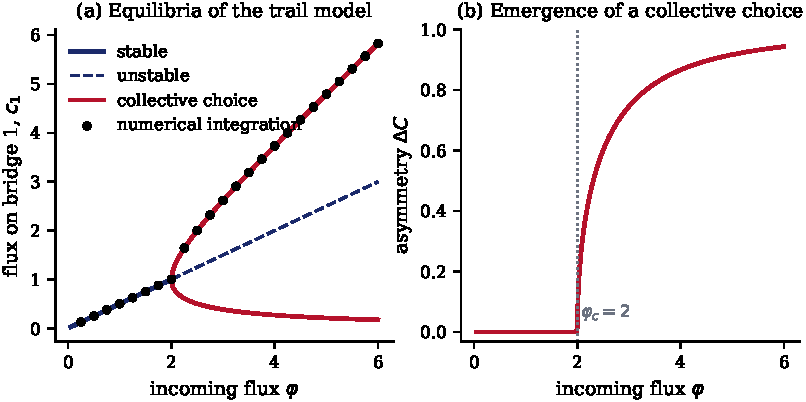
\includegraphics[width=0.58\linewidth]{collective-choice-flow}
  \caption{Flow analysis and the emergence of a collective choice.}
  \label{fig:collective-choice}
\end{figure}

\Cref{fig:collective-choice} shows the traffic flows that produce a collective
choice as a function of the individual deposition amount~$q$. The collective
response (the vertical axis) is indicated by the flow becoming asymmetric over
the two bridges, i.e.,
\begin{equation}
  \Delta C = \frac{\left|C_1 - C_2\right|}{C_1 + C_2}.
  \label{eq:asymmetry}
\end{equation}
A value of $\Delta C > 0$ indicates the emergence of a collective choice.

%-----------------------------------------------------------------------------
\section{Control Architectures for Swarm Robotics}\label{sec:control-architectures}

Control architectures in swarm robotics are designed to achieve robust,
scalable, and flexible collective behavior; they emphasize decentralized
decision-making, lightweight local communication, and formal mechanisms for
convergence and safety in large groups of robots. The central challenge in
swarm control design is that the control paradigm determines how information
flows among the agents and how local interactions produce reliable macroscopic
performance under uncertainty and failures \cite{hamann2018swarm}.

Unlike classical robotics, swarm control favors distributed, self-organized
schemes over monolithic global supervisors, in order to avoid bottlenecks,
single points of failure, and scalability problems with hundreds or thousands of
agents \cite{dias2021swarm}.

\subsection{Decentralized Control}

Decentralized control is the cornerstone of swarm robotics: each robot runs a
simple, autonomous controller that relies on local sensing and neighborhood
exchanges, and macroscopic performance emerges from concurrent local decisions
without a central coordinator \cite{hamann2018swarm,nguyen2024swarm}.

\subsubsection{Local Decision-Making and Adaptability}

In decentralized architectures, each agent perceives only its own
neighborhood, applies local rules, and updates in parallel with its peers; in
this way, behaviors such as flocking, pattern formation, and exploration emerge
without the need for a map or for broadcasting a global state \cite{hamann2018swarm}.
Locality enables rapid adaptation: when the environment or the mission changes,
the agents immediately adapt to the new local cues and drive a coherent
macroscopic reconfiguration without global commands \cite{dias2021swarm}.

A typical local control law for agent $i$ is based on the differences with its
neighbors:
\begin{equation}
  \dot{x}_i = \sum_{j \in \mathcal{N}_i} a_{ij}\,\left(x_j - x_i\right),
  \label{eq:consensus-agent}
\end{equation}
which can be written in vector form as
\begin{equation}
  \dot{x} = -L x,
  \label{eq:consensus-vector}
\end{equation}
where $L$ is the graph Laplacian; convergence is guaranteed under standard
connectivity assumptions \cite{hamann2018swarm}.

Distributed flocking, by combining the simple rules of separation, alignment, and
cohesion, or by imposing geometric constraints, maintains distances, headings,
and shapes using only neighbor data and enables robust motion through unknown
environments \cite{lee2018realtime}.

\subsubsection{Distributed Algorithms and Scalability}

Distributed swarm algorithms emphasize simplicity, locality, robustness, and
parallelism, so that the complexity per robot stays low and performance is
preserved as the team grows \cite{nguyen2024swarm}.

Centralized schemes often suffer from channel congestion and high latency,
whereas distributed protocols naturally balance the load, tolerate faults, and
exploit the concurrency of sensing and actuation \cite{hamann2018swarm}.
\begin{itemize}
  \item \lead{Simplicity and finite state machines} Controllers are often finite
        state machines (FSMs) or short reactive chains, so that their timing
        remains predictable \cite{hamann2018swarm}.
  \item \lead{Local-only communication} Neighbor-to-neighbor exchange preserves
        scalability and avoids saturating a global channel, while still enabling
        consensus, formation, and task allocation over graphs \cite{liu2018virtual}.
  \item \lead{Dynamic membership} Agents may join or leave; the protocols are
        recomputed with the current neighbors and have no hard dependence on
        specific members \cite{dias2021swarm}.
\end{itemize}

\subsubsection{Consensus Principles}

Consensus is the agreement of robots on shared variables---such as reference
frames, headings, goals, virtual leaders, or shape parameters---through local
exchanges over a graph with adjacency matrix $A$ and Laplacian $L$.
Continuous-time average consensus follows $\dot{x} = -Lx$, and its discrete-time
counterpart $x_{k+1} = (I - \varepsilon L)\,x_k$ with step size $\varepsilon$
converges if the graph is connected and the spectral conditions hold \cite{hamann2018swarm}.

Whether in direct, message-based modes or in indirect modes based on density or
motion, consensus is reached on choices such as waypoints or formation branches,
reflecting collective decision-making \cite{hamann2018swarm}.

Practical controllers estimate distributed quantities using local filters,
event-triggered updates, or time-varying weights, in order to reduce bandwidth
and to track changing goals stably and quickly \cite{liu2018virtual}.

An example of event-triggered multi-robot control based on the adjacency matrix
$A = [a_{ij}]$ is
\begin{equation}
  u_i(t) = \sum_{j} a_{ij} \Bigl[\alpha\bigl(x_j(t_j^{s}) - x_i(t_i^{s})\bigr)
           + \beta\bigl(v_j(t_j^{s}) - v_i(t_i^{s})\bigr)\Bigr],
  \label{eq:event-triggered}
\end{equation}
which uses a triggering condition $g_i(t) > 0$ so that each robot updates and
transmits only when necessary, and which guarantees position--velocity consensus
through Lyapunov analysis \cite{liu2018virtual}.

\subsection{Behavior-Based Control Methods}

Behavior-based control (BBC) realizes swarm intelligence through bottom-up
reactive behaviors rather than global plans, keeping the system simple, robust,
and responsive in unknown or dynamic environments \cite{hamann2018swarm}.

BBC is aligned with local sensing/actuation and emergent coordination, which are
hallmarks of scalable swarm operation. Subsumption-style layering prioritizes
behaviors (e.g., obstacle avoidance above exploration): the behaviors run
concurrently, but higher-priority behaviors suppress lower-priority ones and
release them once the stimulus disappears. Iterative refinement at the robot
level---tuning behaviors and thresholds---produces reliable collective patterns
without a global model or explicit global synchronization \cite{nguyen2024swarm}.

\subsubsection{Reactive Behaviors for Emergent Intelligence}

Reactive controllers map the current sensor inputs and a minimal internal state
to actions through condition--action rules and avoid complex world models, so
that they remain replicable across large teams \cite{hamann2018swarm}. Emergent behaviors
such as flocking, dispersion, trail formation, and collective decision-making
arise from many local interactions rather than from a single global planner
\cite{lee2018realtime}.

Artificial potential fields (APFs) superimpose attractive forces toward goals and
repulsive forces from obstacles and peers to provide safe distributed navigation
without global supervision, although parameter tuning and local minima require
care.

\subsubsection{Finite State Machines in Controllers}

FSMs are widely used in swarm controllers: states encapsulate behaviors, and
transitions are triggered by sensor events, timers, or messages, which ensures
predictable responsiveness with a simple architecture \cite{hamann2018swarm}. Probabilistic
FSMs (PFSMs) add stochastic transitions to model noise and variability and
facilitate the analysis of convergence and robustness in aggregation, chaining,
or allocation tasks \cite{hamann2018swarm}.

\subsubsection{Response Threshold Models}

Response threshold models link an agent's probability of switching tasks to the
intensity of a stimulus, producing decentralized and flexible task allocation in
which task sequencing emerges from the accumulation of collective stimuli
\cite{hamann2018swarm}. The standard nonlinearity is
\begin{equation}
  p(s) = \frac{s^{\beta}}{s^{\beta} + \theta^{\beta}},
  \label{eq:response-threshold}
\end{equation}
where $s$ is the stimulus, $\theta$ is the threshold, and $\beta$ controls the
sensitivity. As $s$ exceeds $\theta$, the probability of acting rises sharply,
and coordination emerges without an explicit leader.

\subsection{Hybrid Control Methods}

Hybrid controllers combine behavior-based control with systems-theoretic
guarantees to handle missions that require both fast local responses and
guaranteed macroscopic performance \cite{hamann2018swarm}. A common pattern embeds reactive
rules within a statistical or model-based regulator that governs swarm-level
quantities (e.g., the mean position or the density variance), thereby preserving
autonomy while constraining the macroscopic behavior \cite{hamann2008space}.

This synthesis retains robustness and scalability while achieving explicit
objectives such as tracking, containment, and safety margins through provable
controllers layered around the reactive behaviors.

\subsubsection{Combining Behavior-Based and Systems-Theoretic Approaches}

The goal is to retain the qualitative strengths of BBC---simplicity, robustness,
and fast reaction---while adding formal control to regulate collective metrics
and stability \cite{hamann2018swarm}.

Statistical or macroscopic controllers can constrain the swarm's center of mass
and dispersion, while reactive layers ensure collision avoidance, obstacle
negotiation, and local safety, thus reconciling global guarantees with local
autonomy \cite{hamann2008space}.

Formal tools include Lyapunov functions, graph-theoretic convergence results,
and density-based partial differential equation (PDE) formulations for
quantifying and bounding macroscopic performance under distributed execution
\cite{hamann2018swarm}.

\subsubsection{Applications: Multi-AUV Underwater Missions}

Hybrid control excels underwater, where uncertain currents, limited
communication, and safety-critical sensing require both local reaction and
macroscopic coordination for cooperative target hunting or survey coverage
\cite{liu2018virtual}.

Event-triggered and consensus-based schemes reduce bandwidth while maintaining
formation and tracking, and reactive potential fields provide on-the-spot
avoidance of obstacles and hazards \cite{liu2018virtual}.

In such implementations, the macro layer regulates group objectives (e.g., the
mean trajectory of the formation), while the micro layers execute avoidance,
separation, and target pursuit, so that the autonomy and survivability of each
autonomous underwater vehicle (AUV) are preserved.

A worked example of this layering, cooperative target hunting by a team of
AUVs with an improved potential field, is described in \cref{sec:potential-fields}
\cite{ge2018multi}.

\subsection{Virtual Structure and Virtual Linkage Approaches}

Formation control can be framed as leader--follower, behavior-based, or virtual
structure (VS) control. The virtual linkage (VL) approach generalizes VS to allow
precise control with reconfiguration through virtual joints and links. VL treats
the formation as a mechanical structure of virtual links connected by joints
whose angles determine the shape of the pattern, and it enables reshaping by
controlling the trajectories of these angles \cite{liu2018virtual}.

\subsubsection{Virtual Linkage and Degrees of Freedom}

In VL, the desired shape is parameterized by the virtual joint angles
$\Theta_d$, and the number of joints equals the number of degrees of freedom
available for reconfiguring the pattern; adding an expansion/contraction vector
$\lambda_d$ scales the link lengths for passing through narrow passages. Because
the robots follow only local virtual-linkage references, reshaping is achieved
by broadcasting a small set of parameters to a few link-level controllers, which
reduces communication compared with recomputing the slot of every member
\cite{liu2018virtual}.

VL decouples precise control from global design, offers a compact command space
for frequent changes of shape, and keeps execution distributed at the robot
level. \Cref{fig:virtual-linkage} illustrates how a virtual linkage works.

\begin{figure}[htbp]
  \centering
  \tikzfigure[0.55\linewidth]{virtual-linkage}
  \caption{A mechanical linkage and its virtual counterpart, the virtual linkage
           (redrawn after \cite{liu2018virtual}).}
  \label{fig:virtual-linkage}
\end{figure}

%-----------------------------------------------------------------------------
\section{Communication and Sensing in Swarms}\label{sec:communication}

Communication and sensing are the main channels through which collective
intelligence manifests itself in swarms; local exchange and interaction mirror
the decentralized organization found in nature. The chosen control architecture
fixes the topology of information exchange and hence the performance, so
reliable, fault-tolerant communication is essential for effective coordination
at scale \cite{ge2018multi}.

\subsection{Local Interactions and Limited Communication}

Swarm controllers place decision-making at the agent level and, with simple
computation and minimal sensors on each robot, achieve scalability, robustness,
and flexibility through parallel, neighbor-based interactions. This design
removes any dependence on a global state and keeps working in the presence of
motion, topology changes, and partial failures \cite{dias2021swarm}.

\subsubsection{Local Sensing Capabilities}

Swarm robots are usually homogeneous and resource-constrained, so sensing is
deliberately local and minimal to keep cost and energy consumption low while
still enabling distributed behaviors. Consequently, each robot acts on
instantaneous observations and simple rules, and the range and bearing to nearby
neighbors are vital \cite{dias2021swarm}.
\begin{itemize}
  \item \lead{The need for local sensing} Agents perceive nearby robots and
        obstacles and act autonomously using only these measurements and concise
        rules, which often involve estimating the distances to neighbors for the
        interaction rules.
  \item \lead{Sensor types} Common modalities include proximity and range sensing
        (infrared (IR), ultrasonic), cameras and light sensors, inertial
        measurement units (IMUs), microphones, and simple environmental sensors.
        Very small platforms use IR LEDs and photodiodes for local communication
        and relative localization, and the Kilobot uses downward-facing IR
        reflected off the floor for limited-range communication and localization.
  \item \lead{Purpose} Local sensing makes it possible to follow local rules and
        interact with neighbors, which is essential for decentralized
        coordination and the emergence of group behavior \cite{hamann2018swarm}.
\end{itemize}

\subsubsection{Challenges in Predicting Simultaneous Interactions}

Decentralized swarms face predictability challenges because abundant local
interactions create nonlinear, emergent dynamics that are difficult to control
and predict in advance. This complexity stems from micro-to-macro coupling, in
which macroscopic behavior emerges from microscopic decisions made under limited
information and a changing topology \cite{ge2018multi,hamann2018swarm}.
\begin{itemize}
  \item \lead{Unpredictable emergence} Undesired global patterns can emerge from
        large numbers of simultaneous local interactions, complicating formal
        guarantees and certification.
  \item \lead{Cognitive load} The cognitive difficulty for a human operator does
        not remain a constant $O(1)$; dependencies and incomplete information
        under bandwidth and latency constraints increase the supervision burden.
  \item \lead{Topology dependence} Motion reshapes the graph and risks
        fragmenting it into disconnected components, unless the algorithms
        preserve connectivity and robustness under dynamic neighbor sets.
  \item \lead{Information propagation} Building global maps or shared situational
        awareness from local observations is constrained by short-range,
        limited-bandwidth links and requires efficient multi-hop dissemination in
        highly dynamic networks.
\end{itemize}

\subsubsection{Short-Range Communication}

Swarm design deliberately restricts communication to short ranges to preserve
scalability and robustness by avoiding channel saturation and single points of
failure. Local links enable massive parallelism and redundancy and keep the
hardware of each robot simple and inexpensive \cite{dias2021swarm}.
\begin{itemize}
  \item \lead{Scalability constraint} Global channels scale poorly as the team
        grows, so protocols enforce neighbor-only exchange to keep communication
        costs bounded and decentralized.
  \item \lead{Communication modalities} Both explicit links (peer-to-peer radio)
        and implicit ones (stigmergic or environmental cues, physical contact)
        support distributed coordination under local rules.
  \item \lead{Radio frequency (RF)} IEEE 802.15.4-class radios on platforms such
        as the e-puck are often configured with power control for very short
        ranges (up to a few tens of centimeters) to enforce locality \cite{liu2018virtual}.
  \item \lead{Infrared (IR)} Short-range messaging and proximity sensing,
        including mutual ranging and neighbor discovery, as in the
        s-bot/Swarm-bot systems \cite{sahin2005swarm,liu2018virtual}.
  \item \lead{Sound/ultrasonic} Acoustic links aid localization and messaging and
        can be combined with RF triggering for GPS-free distributed operation on
        land and underwater; the e-puck, for example, carries microphones and a
        speaker that can be used for acoustic messaging \cite{sahin2007swarm}.
\end{itemize}

\subsection{Communication Protocols and Network Topology}

Swarm performance depends strongly on the communication architecture and on the
network topology it induces; together, they determine how information flows, how
quickly consensus forms, and how resilient coordination is to faults. The
co-design of protocol and topology must account for motion-induced changes and
bandwidth constraints in order to maintain stability and throughput \cite{ge2018multi}.

\subsubsection{Decentralized Communication Protocols}

Decentralized protocols allow robots to exchange data without a central broker,
producing robust, scalable, low-latency coordination. The categories include
direct messaging, indirect stigmergy, and direct physical interaction, which are
often combined for redundancy and adaptability \cite{hamann2018swarm,dias2021swarm,ge2018multi}.
\begin{itemize}
  \item \lead{Direct peer-to-peer communication} Explicit exchange of states,
        events, or votes reduces latency and enables rapid reactions to local
        contingencies.
  \item \lead{Indirect communication (stigmergy)} Agents leave environmental
        markers that shape subsequent decisions, providing an inexpensive,
        delay-tolerant flow of information.
  \item \lead{Direct interaction} Physical contact or force sensing conveys local
        state cues and constraints and is useful in tight formations and
        cooperative manipulation.
  \item \lead{Design goals} Local decision-making with adaptive protocols,
        multipath redundancy, and distributed communication functions reduces
        single points of failure and preserves functionality under partial
        outages.
\end{itemize}

\subsubsection{Graph Theory and Network Structure}

Graph theory models robots as nodes and communication links as edges, enabling
analysis based on the adjacency matrix $A$ and the Laplacian $L = D - A$ (where
$D$ is the degree matrix) to support convergence proofs for distributed
controllers. The choice of graph and its connectivity determine the stability
and convergence rates of consensus, formation, and distributed estimation
\cite{hamann2018swarm}.
\begin{itemize}
  \item \lead{Graph types} Undirected graphs model bidirectional exchange and
        directed graphs (digraphs) model one-way flow; the spectral properties of
        $L$ shape the convergence and robustness margins.
  \item \lead{Proximity graphs} The limited sensing and communication range
        induces proximity topologies such as the $r$-disk graph
        $G_{\mathrm{disk}}(r)$, in which an edge exists between two robots that
        are closer than $r$.
  \item \lead{Leader--follower structure} A leader guides the collective motion
        and the followers track it using the leader's state and data from their
        neighbors; convergence in directed networks usually requires a directed
        spanning tree rooted at the leader.
\end{itemize}

\subsubsection{Network-Theoretic Approach to Information Flow}

The network-theoretic perspective views the signaling network of a swarm as a
temporal, adaptive system whose topology co-evolves with the motion of the
agents, coupling communication and control. Information constraints---a limited
capacity $C$ and bandwidth $B$---bound the achievable performance and call for
bandwidth-aware coordination and compression \cite{hamann2008space}.
\begin{itemize}
  \item \lead{Structural properties} Many biological and engineered swarms exhibit
        small-world traits---short paths and high clustering---which support the
        fast and robust propagation of behavioral signals.
  \item \lead{Network controllability} Analysis can identify the minimal set of
        driver agents needed to steer the swarm dynamics and can inform the
        placement of leaders, beacons, or gateway nodes.
\end{itemize}

\subsection{Sensor Models and Data Acquisition}

Sensing, alongside actuation and computation, is a core subsystem; context
awareness is obtained by fusing environmental and inter-agent measurements,
including communication signals interpreted as sensors of the network state. The
key challenge is to fuse heterogeneous, local sensors into robust cooperative
behaviors and shared maps under tight resource constraints \cite{hamann2018swarm,dias2021swarm}.

\subsubsection{Sensor-Based Scene Understanding}

Scene understanding combines representation and data association to produce
actionable context from on-board measurements. Three complementary levels of
representation are common in swarms with heterogeneous payloads and different
roles \cite{dias2021swarm}:
\begin{itemize}
  \item \lead{Appearance level} Local and global visual features support state
        estimation and visual place recognition for lightweight localization.
  \item \lead{Geometry level} LiDAR and RGB-D sensors provide 3-D points and
        depth; RGB-D is sensitive to lighting, whereas LiDAR is costly and heavy,
        which justifies deploying them selectively in mixed swarms.
  \item \lead{Semantic level} Object detection, multi-target tracking, and
        semantic segmentation improve navigation and make simultaneous
        localization and mapping (SLAM) robust to dynamic changes.
  \item \lead{Output artifacts} Semantic local maps and scene graphs provide
        high-level constraints for distributed localization and cooperative
        planning.
\end{itemize}

%-----------------------------------------------------------------------------
\section{Basic Concepts of Path Planning}\label{sec:path-planning-basics}

Path planning is a fundamental problem in robotics and autonomous systems because
it provides the high-level decision-making layer that selects a continuous
sequence of spatial waypoints for the robot to follow, and it directly affects
autonomy, safety, and mission efficiency. In swarm settings, path planning is
intertwined with the decentralized control and communication layers, and it
determines strategic routes that respect local sensing limitations while
optimizing global mission criteria such as time, energy, and robustness
\cite{nguyen2024swarm}.

\subsection{Definition of Path Planning}

Path planning is the problem of computing a feasible---and preferably
optimal---path that moves a robot from an initial state to a goal state in an
environment while respecting geometric, kinematic/dynamic, and safety
constraints. As the field has matured, the goal has shifted from finding ``any
path'' to finding multi-criteria optimal paths that reduce travel time, energy
consumption, and risk, while improving smoothness and robustness for real-world
deployments \cite{nguyen2024swarm}.

\subsubsection{Generating Collision-Free Paths}

A fundamental requirement is collision avoidance: the path must avoid static and
moving obstacles and maintain safety margins along its entire length. In the
configuration-space formulation, complex robot shapes are handled by
``inflating'' the obstacles or ``shrinking'' the robot to a point, so that
collision tests reduce to point-in-free-space checks and an efficient search over
admissible nodes and edges becomes possible \cite{hamann2018swarm}.

Once path planning has delivered a collision-free geometric path, motion planning
assigns time-parameterized velocity and acceleration profiles $v(t)$ and $a(t)$
that are consistent with the dynamic constraints, so that the path is tracked
smoothly and safely. Geometric safety can be enforced by inflating the obstacles
by the robot's footprint, which turns robot--obstacle interference into the
separation of a point from the inflated obstacles in the configuration space
\cite{hamann2018swarm,nguyen2024swarm}.

A typical tracking pipeline optimizes a timing law $s(t)$ along the curve
$\gamma(s)$ so that the bounds $\|\dot{\gamma}\| \le v_{\max}$ and
$\|\ddot{\gamma}\| \le a_{\max}$ are respected, thereby separating spatial
feasibility from dynamic feasibility for embedded controllers \cite{nguyen2024swarm}.

\subsubsection{A Constrained Optimization Problem}

Path planning is a constrained optimization search in which the objective may
combine distance, time, smoothness, energy, and robustness, while feasibility
must respect kinematic, dynamic, and safety constraints; many formulations are
NP-hard in the general case. Multi-objective criteria are common in multi-robot
systems and require Pareto reasoning or scalarization to balance conflicting
objectives, such as the shortest time versus the lowest energy or the largest
safety margin \cite{hamann2018swarm,nguyen2024swarm}.

A representative cost function is
\begin{equation}
  J(\gamma) = \alpha_1 L(\gamma) + \alpha_2 T(\gamma) + \alpha_3 S(\gamma)
              + \alpha_4 E(\gamma),
  \label{eq:cost-function}
\end{equation}
where $L$ is the length, $T$ is the travel time, $S$ is a surrogate for
smoothness such as curvature or jerk, and $E$ is the energy; the coefficients
$\alpha_i$ are tuned to the mission requirements. Swarm intelligence methods such
as PSO and ACO are widely used to approximate global optima under complex
constraints in high-dimensional configuration spaces or dynamic environments,
often smoothing the candidate paths with B-splines to respect nonholonomic
constraints \cite{panigrahi2011handbook}.

\subsection{Global versus Local Planning}\label{sec:global-local}

Planners are classified by the scope of their information: global planners
assume a known map and compute the path from start to end, whereas local
planners act reactively and rely on real-time sensing to cope with unknown or
dynamic obstacles. Practical systems are generally hybrid: global paths serve as
a prior, while local planners ensure safety and reactivity when the map is
incomplete or changes rapidly \cite{hamann2018swarm,nguyen2024swarm}.

\subsubsection{Global Planning}

Given a prior map, global planning computes the complete optimal path from the
origin to the destination, either by discretizing the free space and solving a
graph search or by sampling-based planning that efficiently captures the
connectivity of the space. Classical graph methods such as Dijkstra's algorithm
and \Astar{} guarantee optimality on weighted grids or roadmaps under admissible
heuristics, but they incur replanning overhead when the environment changes
\cite{hamann2018swarm}.

\Astar{} uses a heuristic $h(n)$ with $f(n) = g(n) + h(n)$, and optimality is
preserved when $h$ is admissible and consistent; this is effective for static
maps, but updates are needed when obstacles move. Sampling-based planners such as
the probabilistic roadmap (PRM) and the rapidly-exploring random tree (RRT)
family capture the connectivity of the free space without exhaustive gridding and
scale to high-dimensional configuration spaces, although in their basic forms
they rely on asymptotic rather than exact optimality \cite{nguyen2024swarm}.

\subsubsection{Local Planning}

Local planners rely on on-board sensing to generate admissible motions in real
time and, with minimal model assumptions, focus on obstacle avoidance and
progress toward the goal. Reactive approaches such as artificial potential fields
superimpose an attractive potential toward the goal and repulsive potentials
around the obstacles, providing low-computation navigation; without enhancements,
however, they suffer from local minima and oscillation \cite{bhowmick2024bio}.

The APF law takes the form
\begin{equation}
  U(x) = U_{\att}(x) + U_{\rep}(x),
  \label{eq:apf-basic}
\end{equation}
with the control $u(x) = -\nabla U(x)$. Enhancements include navigation
functions, randomization, and local escape maneuvers to mitigate local minima.
In dynamic scenes, receding-horizon variants and lightweight
velocity-obstacle/optimal reciprocal collision avoidance (ORCA) constraints can
be layered on top of the reactive fields to guarantee collision-free motion while
preserving responsiveness \cite{nguyen2024swarm}.

\subsection{Objectives and Metrics}

Swarm path planning is usually multi-objective: it trades off length, smoothness,
time, energy, and robustness while guaranteeing safety and respecting platform
limitations across many agents. Designing sound metrics is critical, because
swarm missions often lack a single universal optimum and require problem-specific
combinations of objectives and constraints.

\subsubsection{Optimizing Length, Smoothness, and Efficiency}

Minimizing the path length and travel time reduces energy use and improves
throughput, especially when mission duration and battery budgets are tight.
Smoothness is essential for nonholonomic platforms: B-spline or polynomial
smoothing reduces curvature and jerk, so that actuator limits are respected and
tracking errors in motion generation are reduced \cite{panigrahi2011handbook}.

\subsubsection{Maximizing Information Value in UAV Missions}

In unmanned aerial vehicle (UAV) tracking and surveillance, the objectives
emphasize information value, revisit rate, and detection probability while
respecting sensing and communication limits. In passive emitter localization,
the waypoints are optimized to minimize the trace of the Cram\'er--Rao lower bound
(CRLB), yielding favorable time-difference-of-arrival (TDOA) geometries for
accurate estimates under range and angle constraints \cite{nguyen2024swarm}.

Information-driven planning balances observation quality against network
constraints; decentralized model predictive control (MPC) formulations often
maximize the Fisher information or the joint entropy, subject to inter-UAV
spacing constraints that keep communication reliable. CRLB-based planning
constructs sets of waypoints that preserve the observability of the estimator and
a bounded covariance, translating geometry directly into localization-accuracy
objectives \cite{liu2018virtual,nguyen2024swarm}.

\subsubsection{Reducing Computation Time and Energy Consumption}

Real-time swarm deployment demands low computational latency and energy-aware
routing in order to extend mission duration with limited on-board resources.
Energy-oriented planning minimizes the propulsion and sensing/communication
loads, while decentralized receding-horizon methods such as PSO reduce the
solution time and scale to large numbers of agents \cite{panigrahi2011handbook,nguyen2024swarm}.

Decentralized receding-horizon PSO planners have shown performance comparable to
that of centralized methods with far less computation time, enabling on-board
execution and rapid team replanning \cite{panigrahi2011handbook}. In dynamic environments,
RRT-based replanners graft new segments near conflict regions instead of
regenerating the whole path, preserving the optimal segments and reducing CPU
time for rapid collision resolution during motion. ACO-style multi-objective
planners for inspection and coverage tune parameters such as pheromone
evaporation according to energy, achieving sustainability and lower total energy
consumption in long missions \cite{bhowmick2024bio,nguyen2024swarm}.

%=============================================================================
\chapter{Path Planning Algorithms for Swarm Robots}\label{chap:algorithms}
%=============================================================================

This chapter reviews bio-inspired optimization methods that have been adapted for
decentralized, multi-robot path planning, emphasizing their natural inspirations,
their operational rules, and their adaptations to robot collectives for robust
and scalable navigation in dynamic environments.

Swarm intelligence approaches are popular in multi-robot settings because simple
local rules and indirect communication lead to emergent macroscopic behaviors
that remain robust to failures and scale to large populations without
centralized control \cite{nguyen2024swarm}.

%-----------------------------------------------------------------------------
\section{Bio-Inspired Algorithms}\label{sec:bio-inspired}

By mimicking foraging, flocking, and colony organization, bio-inspired algorithms
navigate complex spaces without a global model of the environment, thereby
achieving fast convergence and the ability to escape local minima for NP-hard
combinatorial objectives in multi-robot teams \cite{lin2022review}.

These methods rely on decentralized decisions by the agents, local perception,
and direct interaction or stigmergic signals, which together improve robustness,
scalability, and real-time responsiveness under the uncertainties common in
multi-robot deployments \cite{nguyen2024swarm}. Unlike planners that depend on an
explicit model of the environment, they let each robot act like an individual in
a natural collective, which favors decentralized decisions \cite{chen2025survey}.

\subsection{Ant Colony Optimization (ACO)}

ACO is a classical swarm intelligence method in which artificial ants deposit and
follow pheromone while constructing paths, steering the search toward promising
routes in large combinatorial spaces and in the motion graphs of robots
\cite{panigrahi2011handbook}.

Its core idea is positive feedback through pheromone reinforcement, combined with
evaporation to balance exploitation and exploration, which makes ACO well suited
to high-dimensional routing and discrete motion planning problems in robotics.

\subsubsection{Inspiration from Ant Foraging Behavior}

\begin{itemize}
  \item \lead{Pheromone mechanism} Real ants stochastically prefer paths with
        higher pheromone concentrations, so shorter paths accumulate pheromone
        faster and are chosen more often; the algorithm reproduces these dynamics
        of pheromone deposition and evaporation \cite{panigrahi2011handbook}.
  \item \lead{Stigmergic foundation} Trail laying and trail following constitute
        stigmergy---indirect coordination through modification of the
        environment---which in robotics can be implemented with virtual markers
        or distributed maps for decentralized navigation \cite{yi2019multi}.
\end{itemize}

\begin{figure}[htbp]
  \centering
  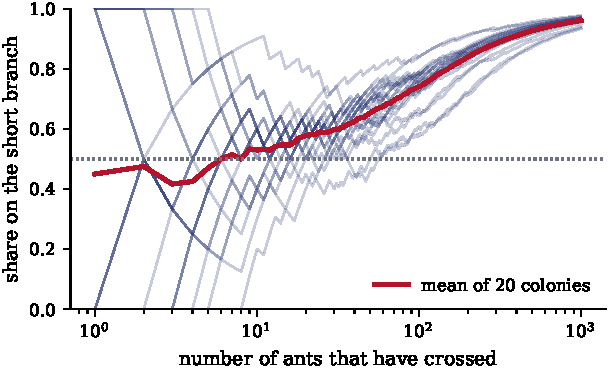
\includegraphics[width=0.72\linewidth]{aco-path-selection}
  \caption{A simulated double-bridge experiment: share of ants on the short
           branch for 20 colonies (thin lines) and their mean (thick line).
           Choices follow \cref{eq:trail-choice} with $k=20$, $\alpha=2$, and the
           long branch is twice as long, so it receives half the pheromone per
           crossing.}
  \label{fig:aco-path-selection}
\end{figure}

\Cref{fig:aco-path-selection} illustrates how ants select paths according to the
pheromone concentration. At first, there is no pheromone on either branch, so the
ants choose at random and the share on the short branch fluctuates around one
half. Because a round trip over the short branch is quicker, it is reinforced
more strongly per unit time (modelled here by a larger deposit), and the
pheromone difference grows. This positive feedback makes later ants prefer the
short branch, and after about a thousand crossings every simulated colony sends
more than 90\% of its traffic over it. These dynamics, which reproduce the
classical double-bridge experiments with real ants \cite{bonabeau1999swarm},
form the basis of ant colony optimization.

\subsubsection{Variants and Applications (AS-TSP, ACS-TSP)}

\begin{itemize}
  \item \lead{Ant System (AS-TSP)} The first ACO algorithm, proposed for the
        traveling salesman problem (TSP), which introduced the pheromone-guided
        constructive building of solutions but was later surpassed by improved
        variants \cite{dorigo1996ant}.
  \item \lead{Ant Colony System (ACS-TSP)} ACS strengthens AS with local pheromone
        updates, usually integrates local search such as 2-opt and 3-opt, and
        achieves leading performance, especially on the asymmetric TSP
        \cite{dorigo1997ant,bonabeau1999swarm}.
  \item \lead{Other applications} ACO variants have addressed quadratic
        assignment, sequential ordering, vehicle routing, and graph coloring
        problems. In robotics, ACO has been used to optimize the parameters of
        the membership functions of fuzzy controllers and, combined with fuzzy
        cost functions, for the navigation and path planning of mobile robots
        \cite{panigrahi2011handbook}. Together with PSO, ACO was one of the two
        mainstream paradigms of early swarm-intelligence research
        \cite{seebacher2025collective}.
\end{itemize}

\subsubsection{Pheromone Update Rules and Heuristics}

In standard ACO on graphs, a probabilistic transition rule weights the pheromone
intensity $\tau$ and the heuristic desirability $\eta$; pheromone evaporation and
a deposition proportional to the quality of the tour are then applied:
\begin{align}
  p_{ij}^{k}(t) &=
    \begin{cases}
      \dfrac{\tau_{ij}(t)^{\alpha}\,\eta_{ij}^{\beta}}
            {\sum_{u \in \mathcal{N}_i^{k}} \tau_{iu}(t)^{\alpha}\,\eta_{iu}^{\beta}},
        & j \in \mathcal{N}_i^{k}, \\[2ex]
      0, & \text{otherwise},
    \end{cases}
    \label{eq:aco-transition} \\[1ex]
  \eta_{ij} &= \frac{1}{d_{ij}},
    \label{eq:aco-heuristic} \\[1ex]
  \tau_{ij}(t+1) &= (1-\rho)\,\tau_{ij}(t) + \sum_{k=1}^{m} \Delta\tau_{ij}^{k},
    \label{eq:aco-update} \\[1ex]
  \Delta\tau_{ij}^{k} &=
    \begin{cases}
      \dfrac{Q}{L_k}, & \text{if } (i,j) \text{ is in the tour of ant } k, \\[1.5ex]
      0, & \text{otherwise}.
    \end{cases}
    \label{eq:aco-deposit}
\end{align}

In ACS, a local update that decreases the pheromone after each move lowers the
pheromone on recently used edges, which encourages exploration and prevents
premature stagnation \cite{panigrahi2011handbook}.

\subsubsection{Theoretical Aspects and Runtime Analysis}

\begin{itemize}
  \item \lead{Construction-graph model} ACO can be modeled as the construction of
        solutions on a graph with restricted transition neighborhoods and
        stochastic selection, which allows probabilistic runtime bounds to be
        derived, for example through fitness-level arguments
        \cite{gutjahr2007mathematical}.
  \item \lead{Convergence} Formal results show that the pheromones are bounded
        and that, with sufficient iterations and suitable parameter ranges, the
        probability of sampling optimal tours is positive; probabilistic
        convergence is thereby established for the basic ACO models
        \cite{gutjahr2007mathematical}.
  \item \lead{Controller tuning} Grid-based ACO has been used to tune the
        parameters of nonlinear PID (NLPID) controllers, and its convergence has
        been demonstrated in simulation loops for mechatronic systems, which
        illustrates the synergy between control and optimization
        \cite{panigrahi2011handbook}. The corresponding block diagram is shown in
        \cref{fig:aco-nlpid}.
\end{itemize}

\begin{figure}[htbp]
  \centering
  \tikzfigure[0.88\linewidth]{aco-nlpid}
  \caption{Using ACO to tune the parameters of an NLPID controller (redrawn after
           \cite{panigrahi2011handbook}).}
  \label{fig:aco-nlpid}
\end{figure}

\subsection{Particle Swarm Optimization (PSO)}

PSO models a swarm of particles that update their velocities and positions by
combining inertial motion, their personal best experience, and the social best,
yielding a simple yet powerful optimizer with strong empirical convergence and
low computational overhead \cite{nguyen2024swarm}.

Compared with many heuristics, PSO requires few parameters, is inherently
parallelizable, and is effective for continuous trajectory parameterization,
controller tuning, formation shaping, and multi-robot task allocation \cite{chen2019path}.

\subsubsection{Inspiration from Bird Flocking and Fish Schooling}

PSO was proposed by Kennedy and Eberhart in 1995 as a model of the social
behavior of bird flocks and fish schools \cite{kennedy1995particle}. Each particle
is a candidate solution in the search space, and its motion combines its current
velocity, the best position it has found itself (the personal best $p_i$), and
the best position found by the swarm or its neighborhood (the global best $g$).
This cognitive--social mechanism reflects alignment and cohesion in flocks and
schools, while inertia supports exploration
\cite{nguyen2024swarm,poli2007particle}:
\begin{equation}
  v_i^{t+1} = w\,v_i^{t} + c_1 r_1\left(p_i - x_i^{t}\right)
              + c_2 r_2\left(g - x_i^{t}\right), \qquad
  x_i^{t+1} = x_i^{t} + v_i^{t+1}, \qquad
  r_1, r_2 \sim U(0,1).
  \label{eq:pso}
\end{equation}

\subsubsection{Variants and Improvements (IPSO-DAI, NisB PSO)}

\begin{itemize}
  \item \lead{Parameter scheduling} Linearly decreasing the inertia weight $w$
        improves global exploration early in the search and local exploitation
        later on, reducing the risk of premature convergence in complex
        landscapes \cite{chen2019path}.
  \item \lead{PSO with integral control (IPSO-DAI)} Integral-controlled PSO
        (ICPSO) adds two integral controllers to the update to keep the
        population diverse; IPSO-DAI extends it with dispersed accelerator
        information, so that a predicted velocity index decides whether a particle
        moves in a divergent or a convergent manner. On high-dimensional
        multimodal benchmarks with many local optima, it outperformed standard
        PSO and ICPSO \cite{panigrahi2011handbook}.
  \item \lead{Topology} Ring topologies (lbest PSO) restrict the social
        neighborhood, and niching splits the swarm into sub-swarms (e.g., kPSO
        and NichePSO) that maintain multiple optima for multimodal path planning
        and multi-objective missions \cite{panigrahi2011handbook}; the robotic
        Darwinian PSO (RDPSO) uses the same idea of smaller sub-swarms to escape
        local optima with real robots \cite{dias2021swarm}.
  \item \lead{Hybrids} Combining PSO with B-spline smoothing, gravitational search,
        or symbiotic search improves compliance with kinematic/dynamic
        constraints and enhances the smoothness of solutions for flight and
        driving paths.
  \item \lead{Oscillating and collision-free PSO} Adding second-order/oscillatory
        terms together with collision-free constraints keeps the particles inside
        the feasible region in constrained navigation domains.
\end{itemize}

\subsubsection{Multi-Objective PSO (MOPSO)}

MOPSO generalizes single-objective PSO by replacing the single global best $g$
with archives of non-dominated solutions and with crowding or clustering
criteria that maintain a diverse Pareto front; it also redefines how the guides
for $p_i$ and for the group are selected, since with conflicting objectives there
is no single best position \cite{panigrahi2011handbook}. Representative variants
include:
\begin{itemize}
  \item \lead{Adaptive MOPSO (AMOPSO)} The inertia and acceleration coefficients
        are adapted over the iterations.
  \item \lead{Constrained adaptive MOPSO (CAMOPSO)} A penalty-based mechanism lets
        marginally infeasible solutions return to the feasible region, which
        helps when the feasible space is disconnected.
  \item \lead{Non-dominated sorting PSO (NSPSO)} Non-dominated sorting is used to
        rank the swarm and manage the front.
  \item \lead{Clustering} Clustering bounds the size of the archive and keeps the
        stored Pareto set well distributed.
\end{itemize}
A MOPSO generates a whole set of non-dominated solutions in one run, after which
fuzzy decision-making can pick the best compromise \cite{panigrahi2011handbook}.

\subsubsection{Application to UAV Swarm Path Planning}

\begin{itemize}
  \item \lead{Optimal paths} PSO plans short and safe paths for multiple vehicles
        while respecting obstacle and mission-time constraints; PSO formulations
        for simultaneous arrival and for minimizing mission time are common in
        multi-UAV scenarios \cite{he2021novel}. An example is shown in
        \cref{fig:pso-path}.
  \item \lead{Distributed control and reconnaissance} PSO updates have been used
        directly as the position commands of real quadcopters in swarm search
        \cite{lee2018realtime}; cooperative PSO generates safe, flyable paths for
        multi-UAV rendezvous that respect kinematic limits and are often smoothed
        with B-splines for curvature continuity \cite{lin2022review}.
  \item \lead{Controller and parameter tuning} Two-layer PSO frameworks tune the
        parameters of an inner target-tracking loop, while an outer loop
        optimizes the inner gains, enabling rapid gain synthesis across many
        geometric paths.
  \item \lead{Benchmarking} PSO is a standard baseline for comparison with newer
        bio-inspired methods (such as pigeon-inspired optimization) in aerial
        planning \cite{tan2016handbook,lin2022review}.
\end{itemize}

\begin{figure}[htbp]
  \centering
  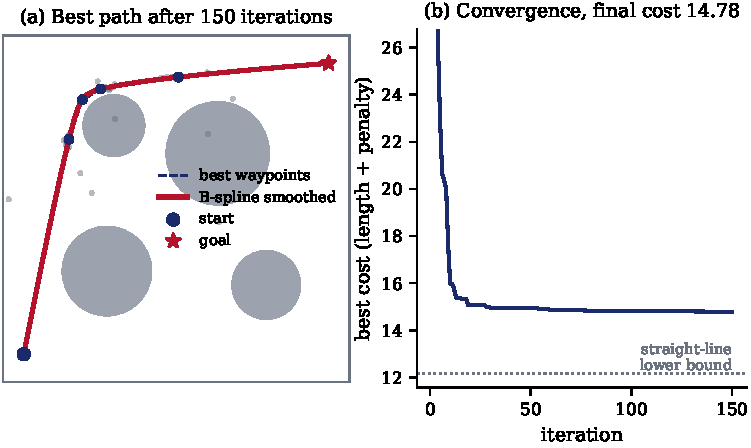
\includegraphics[width=\linewidth]{pso-path-planning}
  \caption{PSO path planning: each particle encodes four waypoints between the
           start and the goal, and the cost is the path length plus a penalty for
           entering an inflated obstacle. (a) The best waypoints after 150
           iterations, smoothed with a cubic B-spline; the grey dots are the final
           positions of the swarm. (b) Convergence of the best cost.}
  \label{fig:pso-path}
\end{figure}

\subsection{Bee-Inspired Algorithms}

Bee-inspired approaches mimic the division of labor and the recruitment of
foragers through waggle-dance-like communication in order to balance exploration
(scouts) and exploitation (employed and onlooker bees), producing robust global
search dynamics with few hyperparameters \cite{liang2015efficient}.

Honey-bee-based frameworks also include honey bee mating optimization (HBMO), the
Bees Algorithm (BA), and bee-colony-inspired methods tailored to discrete
constraints (e.g., time windows) in logistics \cite{liang2015efficient}.

\subsubsection{Honey Bees and the Artificial Bee Colony (ABC)}

ABC \cite{karaboga2005idea} divides the agents into employed bees (attached to food
sources, i.e., the current solutions), onlookers (which select sources
probabilistically according to their fitness), and scouts (which perform random
exploration or re-initialization after an abandonment limit is reached); with the
colony size and the number of cycles as its main control parameters, it delivers
robust performance \cite{panigrahi2011handbook}.

Its advantages include simplicity, robustness, and a small set of parameters,
although the search can slow down near the optimum and diversity can decrease.
Variants such as BCiA (for the vehicle routing problem with time windows,
VRP-TW) and BA (for training neural networks) adjust the balance between
exploration and exploitation and the problem encoding for discrete settings
\cite{panigrahi2011handbook}.

\subsubsection{Hierarchical and Multi-Island ABC Models}

Parallel and distributed ABC variants, by offloading evaluations, sharing elite
solutions, and co-evolving subpopulations, improve the scalability of
high-dimensional path planning, reducing the wall-clock time while preserving
diversity \cite{panigrahi2011handbook}.
\begin{itemize}
  \item \lead{Master--worker ABC} Central coordination parallelizes costly
        evaluations and local searches on worker nodes to accelerate
        time-critical planning \cite{panigrahi2011handbook}.
  \item \lead{Multi-hive (multi-island) ABC} Independent hives periodically
        migrate elite solutions and, through co-evolution, raise the quality of
        the solutions while containing the growth of computation
        \cite{panigrahi2011handbook}.
  \item \lead{Hierarchical--hybrid ABC (HH-ABC)} Islands exchange elites at the
        upper level, and each island internally runs a master--worker ABC,
        combining diversification with parallel speedup at large scale
        \cite{panigrahi2011handbook}.
\end{itemize}
In comparisons with an enhanced sequential ABC that also uses local search, the
parallel and multi-population models consistently reached good solutions with
less computation on problems with many variables \cite{panigrahi2011handbook}.

\subsection{Other Swarm Intelligence Algorithms}

Many other natural metaphors have produced metaheuristics that are used for
high-dimensional planning and optimization in swarm robotics
\cite{shahzad2023review,nguyen2024swarm}.

\subsubsection{Firefly, Flower Pollination, and Artificial Flora Algorithms}

In the firefly algorithm (FA), the brightness of a firefly encodes the quality of
its solution, and a dimmer firefly moves toward a brighter one, so the
population gathers around the best individual \cite{yang2009firefly}. A common
form of the update is
\begin{equation}
  x_i \leftarrow x_i + \beta_0\, e^{-\gamma r_{ij}^{2}} \left(x_j - x_i\right)
        + \alpha\, \epsilon_i,
  \label{eq:firefly}
\end{equation}
where $r_{ij}$ is the distance between fireflies $i$ and $j$, $\beta_0$ is the
attractiveness at zero distance, $\gamma$ is the light absorption coefficient,
and the random term $\alpha \epsilon_i$ keeps the search from stagnating. The
flower pollination algorithm (FPA) imitates the global and local pollination of
flowering plants \cite{yang2012flower}, and the related artificial flora (AF)
algorithm imitates how plants spread seeds over an area to find the best place to
grow, generating ``offspring plants'' around an ``original plant'' with
propagation functions; in its authors' comparisons, AF was more stable and
accurate than PSO and ABC \cite{cheng2018artificial}.

\subsubsection{Fireworks and Dragonfly Algorithms}

The fireworks algorithm (FWA), introduced by Tan, models the explosion of
fireworks: good solutions act as explosion sites around which ``sparks''
(new candidate solutions) are generated to refine the search \cite{tan2010fireworks}.
The guided fireworks algorithm reappears in \cref{sec:learning} as the optimizer
of a learned search policy. The dragonfly algorithm imitates the static and
dynamic swarming of dragonflies \cite{mirjalili2016dragonfly}, and its strategy
parameters have been tuned to make multi-target search by robot swarms more
efficient \cite{bhowmick2024bio}.

\subsubsection{Glowworm Swarm Optimization (GSO)}

GSO is designed for multimodal problems in which several optima, or several
sources, must be found at once. Each glowworm carries a luminescence quantity,
\emph{luciferin}, which grows with the fitness $J$ at its position and decays
over time,
\begin{equation}
  \ell_i(t+1) = (1-\rho)\,\ell_i(t) + \gamma\, J\bigl(x_i(t+1)\bigr),
  \label{eq:gso}
\end{equation}
and each agent moves toward a brighter neighbor within an adaptive decision
range. Because distant individuals have no influence, the swarm splits
automatically into sub-swarms around the different optima. GSO has been used
for localizing multiple odor sources and tracking mobile signal sources with
groups of robots \cite{krishnanand2009glowworm,panigrahi2011handbook}.

\subsubsection{Distributed Hybrid Fish Swarm Optimization (DHFSOA)}

DHFSOA is an example of the trend toward specialized, hybrid swarm algorithms.
Based on the collective search of fish schools, it was proposed for event-driven
sensor deployment in underwater acoustic sensor networks, where conventional
redeployment algorithms become complicated, and it finds good deployments faster
than traditional methods \cite{wang2018event}.

%-----------------------------------------------------------------------------
\section{Graph-Based and Sampling-Based Methods}\label{sec:graph-sampling}

Graph- and sampling-based planners convert continuous motion planning into a
tractable discrete search by building graphs or trees in the free space; this
approach is particularly effective in high-dimensional or geometrically complex
environments, where cell grids or potential fields struggle \cite{abujabal2024path}.

These methods offer probabilistic completeness or strong practical performance
while remaining compatible with the decentralized execution that is common in
swarms \cite{lin2022review}.

\subsection{Probabilistic Roadmap (PRM)}

PRM is a classical multi-query sampling-based planner that builds a roadmap of
sampled collision-free configurations and connects them with local planners; it
then links the start and goal points to the roadmap and finds a path through
graph search \cite{kavraki1996probabilistic}. Its multi-query nature and
relatively low query cost have made PRM a common backbone that is combined with
metaheuristics or behavioral rules in multi-robot systems and swarms
\cite{neto2017multi,lin2022review}. Complete planners, which find a path or prove
that none exists, need time that grows exponentially with the number of degrees
of freedom, which is why randomized methods such as PRM are preferred in high
dimensions \cite{kavraki1996probabilistic}.

\subsubsection{Roadmap Construction in High-Dimensional Spaces}

PRM tames the exponential growth of the configuration space with increasing
degrees of freedom by random sampling, approximating the connectivity of $\Cfree$
without an exhaustive search. The pipeline has two phases: a preprocessing phase,
which builds the roadmap by sampling collision-free milestones and connecting
nearby neighbors with a simple local planner, and a query phase, which connects
the start and goal to the roadmap and runs a graph search for a feasible path
\cite{neto2017multi}.

The roadmap approximates a graph over $\Cfree$ whose vertices are the milestones
and whose edges are feasible local connections; its completeness is
probabilistic and improves with the number of samples and the connection radius
\cite{neto2017multi}.
\begin{itemize}
  \item \lead{Managing complexity} Performance depends on the number and
        placement of the milestones; informed samplers such as Medial-Axis PRM
        (MAPRM) bias the samples toward the medial axis to increase safety
        margins, yielding higher-quality roadmaps with fewer samples
        \cite{sahin2005swarm}.
\end{itemize}

\begin{figure}[htbp]
  \centering
  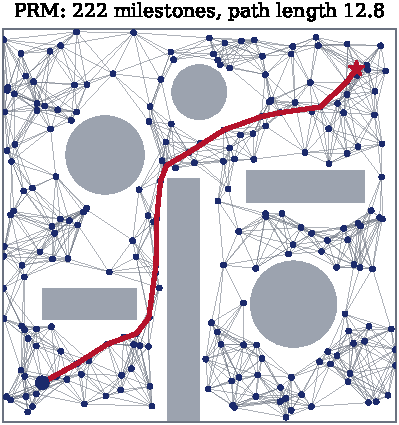
\includegraphics[width=0.55\linewidth]{prm-example}
  \caption{PRM in a cluttered workspace: collision-free milestones are connected to
           their ten nearest neighbours, and Dijkstra's algorithm finds the path on
           the roadmap.}
  \label{fig:prm}
\end{figure}

\subsubsection{Integration with Flocking and Shepherding}

Roadmaps inject a global navigation structure into swarms that interact mainly
locally, enabling coordinated homing, exploration and coverage, passage through
narrow corridors, and shepherding strategies.\footnote{Shepherding: an external
agent selects a path on the roadmap and, by issuing commands, guides the swarm
along it, so that global guidance is blended with the local cohesion of the
flock \cite{sahin2005swarm}.} Flocks can traverse the edges of the roadmap while node-level
rules for separation, alignment, and cohesion preserve the formation and spacing,
especially in narrow regions or bottlenecks \cite{sahin2005swarm}. Roadmaps have
supported several group behaviors:
\begin{itemize}
  \item \lead{Homing and goal searching} The roadmap gives the flock the
        structure it needs to reach a known goal or to search for an unknown one.
  \item \lead{Exploration and coverage} The edges gain weight as robots traverse
        them, and at each junction the flock chooses probabilistically in favor of
        lower-weight edges, so less-visited corridors get priority.
  \item \lead{Narrow passages} Roadmap nodes can carry rules that the flock
        members apply when they reach them, which coordinates the flock's
        configuration in narrow or complex areas.
  \item \lead{Shepherding} An external agent extracts a path from the roadmap and
        steers the flock from behind along it.
\end{itemize}

\subsection{Rapidly-Exploring Random Trees (RRT)}

RRT samples the state space and greedily extends a tree from the nearest node
toward each sample, rapidly exploring unknown regions and quickly producing
feasible (though not necessarily optimal) paths
\cite{lavalle1998rapidly,abujabal2024path}.

RRT is probabilistically complete and accommodates kinodynamic constraints, which
makes it practical for robots with dynamics and control limitations.

\subsubsection{RRT and RRT-Connect for Single-Agent Queries}

RRT views motion planning as a tree search that expands toward uniform samples
and connects new states to their nearest neighbor using a local steering function
subject to the constraints \cite{lavalle1998rapidly}.

RRT-Connect grows two trees, one from the start and one from the goal, and
aggressively attempts to join them with its CONNECT heuristic, which reduces the
search time compared with a single tree \cite{kuffner2000rrt}. \RRTstar{} adds a
rewiring step that makes the solution asymptotically optimal, at a higher
computational cost \cite{karaman2011sampling}. The difference between RRT and
RRT-Connect can be seen in \cref{fig:rrt}.

\begin{figure}[htbp]
  \centering
  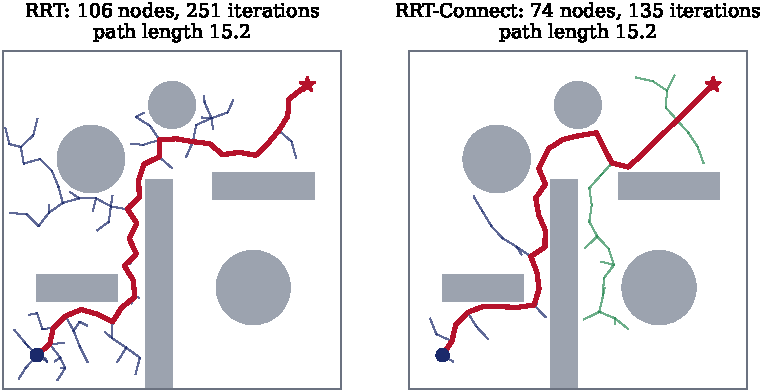
\includegraphics[width=0.95\linewidth]{rrt-vs-rrt-connect}
  \caption{RRT and RRT-Connect in the workspace of \cref{fig:prm}, with the same
           step size and random seed. RRT-Connect grows a tree from each end and
           joins them with its CONNECT step, so it needs fewer iterations.}
  \label{fig:rrt}
\end{figure}

\subsubsection{Adaptations for Swarm Robotics (e.g., Virtual Tubes)}

Distributed RRT enables decentralized collision avoidance: each agent plans while
accounting for the other agents and the static obstacles, using local
communication when needed \cite{lin2022review}.

In dynamic environments, \emph{grafting}---inserting new intermediate waypoints
into an existing RRT path when the obstacles change---avoids complete replanning
and enables real-time updates for multi-robot teams \cite{li2021rrt}.
\begin{itemize}
  \item \lead{Optimal virtual tube planning (OVTP) and Tube-\RRTstar} A
        hierarchical approach first generates homotopic paths (e.g., with
        \RRTstar) and then builds an ``optimal virtual tube'' that bounds safe,
        obstacle-free corridors for the synthesis of a central path and for
        distributed execution; Tube-\RRTstar{} trades off path length against the
        cross-sectional area of the corridor in order to contain the swarm
        \cite{mao2023optimal,mao2024tube}.
\end{itemize}
The computational complexity of tube planning is
\begin{equation}
  O\bigl(n(\log n + 1) + l\bigr),
  \label{eq:tube-complexity}
\end{equation}
for $l$ homotopic paths on $n$ samples, compared with
\begin{equation}
  O\bigl(n\,l\,(\log n + 1)\bigr)
  \label{eq:multipath-complexity}
\end{equation}
when \RRTstar{} is simply run $l$ times \cite{mao2024tube}.

\subsubsection{Sub-Optimal Algorithms for Higher Speed}

\begin{itemize}
  \item \lead{Multi-tree structures} Bidirectional RRT-Connect and three-tree
        approaches parallelize exploration from multiple fronts and improve the
        success rate in narrow passages \cite{abujabal2024path,yuan2020bilevel}.
  \item \lead{Biased sampling} Goal biasing accelerates convergence;
        obstacle-biased methods (e.g., Dangerzone RRT) steer the samples toward
        the boundaries of obstacles so that narrow corridors are traversed
        efficiently.
  \item \lead{Roadmap-guided sampling} GVD-guided RRT uses the generalized
        Voronoi diagram (GVD) as a heuristic backbone and greatly accelerates
        planning in maze-like scenes.
  \item \lead{Dynamic replanning} DRRT prunes and repairs only the invalidated
        parts of the path when changes occur; ERRT resumes growth when the path
        is blocked; and multipartite RRTs (MPRRT) combine fast pruning with
        restart behavior to maintain responsiveness \cite{chen2025survey}.
  \item \lead{Pseudo-random trees} The multi-agent rapidly-exploring pseudo-random
        tree replaces random sampling with a deterministic sequence, keeping
        probabilistic completeness while converging quickly
        \cite{neto2017multi}.
\end{itemize}

\subsection{The \texorpdfstring{\Astar}{A*} Algorithm and Grid-Based Methods}

Deterministic graph and grid planners are fundamental for structured maps:
\Astar{} yields optimal paths with the help of heuristics, and grids and cell
decompositions provide discrete models that are suited to proofs of correctness
and to integration with other planners. These methods are often used as
baselines or as components of hybrid multi-robot path planning systems
\cite{abujabal2024path,lin2022review}.

\subsubsection{\texorpdfstring{\Astar}{A*} for Optimal Paths in Static Environments}

\Astar{} evaluates nodes with $f(n) = g(n) + h(n)$, where $g(n)$ is the cost from
the start and $h(n)$ is an admissible heuristic estimate of the cost to the goal;
this guarantees completeness and optimality on graphs with nonnegative edge
weights \cite{hart1968formal}. An example of how this method works is shown in
\cref{fig:astar}; its weakness is that the search effort still grows quickly as
the search space expands \cite{abujabal2024path}.

With informed heuristics, \Astar{} is more efficient than Dijkstra's algorithm in
large spaces, and it is often combined with fuzzy neural networks to speed up
task completion and improve controllability and adaptability in multi-robot
systems \cite{tan2016handbook}.

\begin{figure}[htbp]
  \centering
  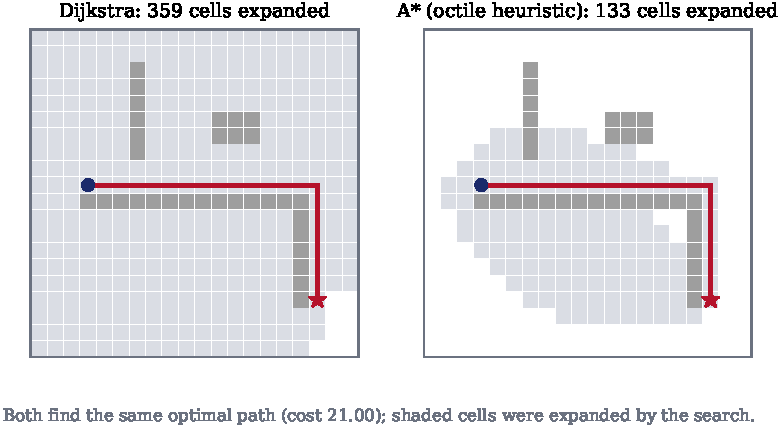
\includegraphics[width=0.9\linewidth]{astar-grid}
  \caption{Dijkstra's algorithm and \Astar{} on the same 8-connected grid. Both
           return the same optimal path, but the admissible octile heuristic lets
           \Astar{} expand far fewer cells.}
  \label{fig:astar}
\end{figure}

\subsubsection{Grid-Based Environment Representation}

Grid maps discretize space into cells, turning continuous motion into a graph
search for algorithms such as \Astar, \Dstar, or even ACO on grids, and they can
be updated online to handle dynamics \cite{abujabal2024path}. The resolution is a critical
trade-off between accuracy and computation or memory: a very fine grid is
expensive and a very coarse one is inaccurate, which is why multi-resolution or
hierarchical grids are attractive in practice \cite{lin2022review}.

\subsubsection{Cell Decomposition Techniques (e.g., Boustrophedon, Morse)}

Cell decomposition partitions $\Cfree$ into non-overlapping cells and builds an
adjacency graph whose nodes are the cells and whose edges are adjacency
relations; optimal paths are obtained by a graph search across the cells with
methods such as Dijkstra's algorithm or \Astar{} \cite{abujabal2024path}.

Boustrophedon decomposition supports exact coverage by sweeping and splitting the
space at points where its connectivity changes \cite{choset2000coverage}, whereas
Morse decompositions use the critical points of a Morse function to produce cells
that are easily covered with simple back-and-forth patterns once entered
\cite{acar2006sensor}.

\subsubsection{Generalized Voronoi Diagrams (GVD) for Narrow Regions}

The GVD partitions the free space into loci that are equidistant from the
obstacles: its edges are the points equidistant from two obstacles, and its meet
points are equidistant from three or more. By maximizing the safety margin, these
edges and junctions serve as a roadmap for safe passage through cluttered
environments and narrow passages \cite{acar2006sensor,breitenmoser2010voronoi}.

Planning can move along the GVD, reach its edges near the goal, and then exit
toward the goal. The GVD also guides sensor-based coverage, accelerates RRT in
maze-like environments, and supports path-priority strategies for multiple robots
in narrow passages \cite{breitenmoser2010voronoi}.

\begin{figure}[htbp]
  \centering
  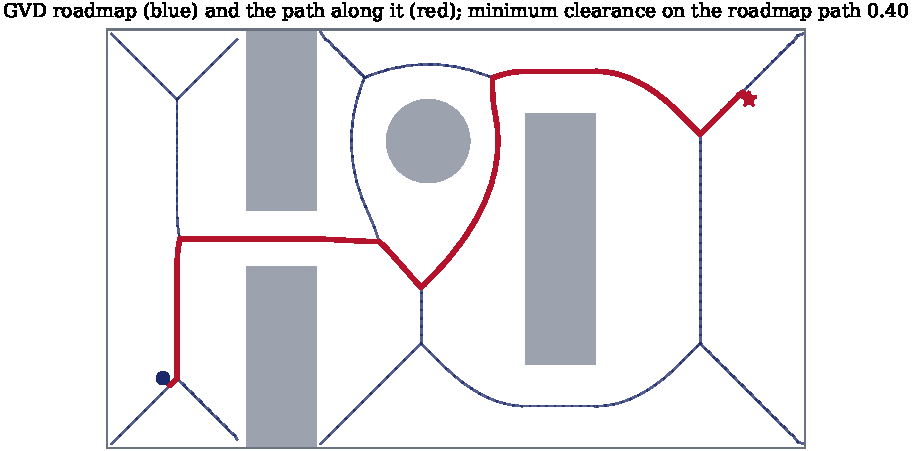
\includegraphics[width=0.85\linewidth]{voronoi-narrow-regions}
  \caption{An approximate generalized Voronoi diagram, built from the ordinary
           Voronoi diagram of points sampled on the obstacle boundaries. The path
           follows the roadmap through the narrow door and keeps the largest
           possible distance from the walls.}
  \label{fig:voronoi}
\end{figure}

%-----------------------------------------------------------------------------
\section{Potential Field Methods}\label{sec:potential-fields}

Potential field planners, and particularly the artificial potential field (APF),
turn path planning into gradient-following motion by defining deterministic,
rule-based potentials. Their simplicity, fast computation, and real-time
reactivity in dynamic scenes make them attractive for distributed swarms
\cite{nazarahari2019multi}.

In multi-robot systems, the APF is usually employed as a local planner or control
law that integrates smoothly with higher-level graph or sampling planners or with
metaheuristics, keeping the computational cost per agent low while preserving
decentralized execution \cite{wang2022coordination}.

\subsection{Artificial Potential Fields (APF)}

The APF, pioneered by Khatib in 1986, remains the standard for geometric
navigation based on force fields: the goal creates attraction in the
configuration space, the obstacles create repulsion, and the motion commands are
derived from the negative gradient of the potential \cite{khatib1986real}.

In multi-agent settings, the APF models inter-agent and agent--environment
interactions as attractive--repulsive potentials, and gradient-based controls
ensure formation, tracking, and collision avoidance with decentralized feedback
\cite{wang2018research}.

\subsubsection{Attractive and Repulsive Forces for Navigation}

The APF defines a total potential $U(X)$ as the sum of attractive and repulsive
components and computes the net control force as the negative gradient of this
potential, so that the robot descends toward the goal while keeping away from the
obstacles:
\begin{equation}
  U(X) = U_{\att}(X) + U_{\rep}(X), \qquad
  F(X) = -\nabla U(X) = F_{\att}(X) + F_{\rep}(X).
  \label{eq:apf}
\end{equation}
Here, $U_{\att}$ pulls the agent toward the goal, and $U_{\rep}$ increases sharply
near the obstacles to preserve safety, providing smooth closed-loop motion that
is suitable for real-time embedded control \cite{wang2022coordination}. A common
attractive potential is quadratic, $U_{\att}(X) = \tfrac{1}{2} k_{\att}
\|X - X_g\|^2$, and a typical repulsive potential is
\begin{equation}
  U_{\rep}(X) =
  \begin{cases}
    \dfrac{1}{2}\,k_{\rep}\left(\dfrac{1}{d(X)} - \dfrac{1}{d_0}\right)^{2},
      & d(X) \le d_0, \\[2.5ex]
    0, & d(X) > d_0.
  \end{cases}
  \label{eq:apf-repulsive}
\end{equation}
Consequently, $\|\nabla U_{\rep}\|$ grows without bound as $d(X) \to 0$, which
gives priority to collision avoidance near the boundaries \cite{zhao2020multi}.

\begin{figure}[htbp]
  \centering
  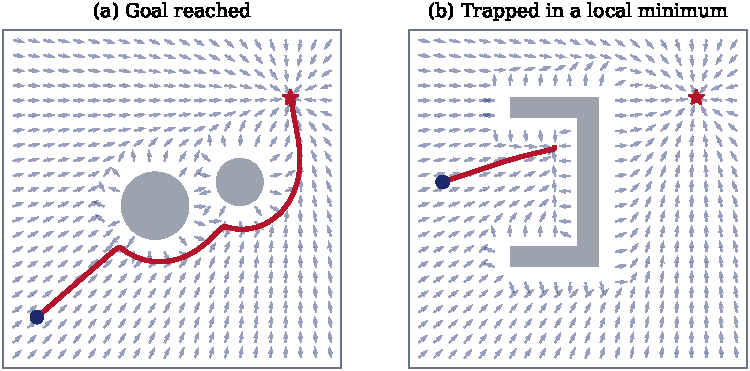
\includegraphics[width=\linewidth]{apf-forces}
  \caption{The force-field view of robot path planning: the arrows show the
           direction of $F = -\nabla U$. (a) The target attracts and the
           obstacles repel the robot, which reaches the goal. (b) A U-shaped
           obstacle creates a local minimum in which the same controller gets
           stuck.}
  \label{fig:apf}
\end{figure}

\subsubsection{Principles of Obstacle Avoidance and Goal Seeking}

\begin{itemize}
  \item \lead{Goal seeking} $U_{\att}(X)$ is shaped so that the magnitude of the
        attractive force is large far from the goal and zero at the goal; this
        ensures natural deceleration and stopping at the potential minimum and
        encodes precise capture of the goal in static scenes \cite{wang2022coordination}.
  \item \lead{Obstacle avoidance} $U_{\rep}(X)$ grows rapidly as the distance to
        the obstacles decreases and can vanish outside a radius of influence;
        this design enforces separation because the repulsive gradient dominates
        near the boundaries \cite{wang2018research}.
  \item \lead{Known limitations} The classical APF may suffer from local minima
        and is sensitive to parameter tuning, which can trap the robot away from
        the global minimum; hybridization or adaptive shaping is commonly used in
        practice to mitigate this problem \cite{zhao2020multi}.
\end{itemize}

\subsubsection{Improved Potential Field for Cooperative Target Hunting}

To overcome local minima and embed multi-robot cooperation, improved potential
fields (IPFs) add cooperation measures and problem-specific shaping, which enables
coordinated target hunting by multi-AUV teams in turbulent, dynamic surface-water
environments \cite{ge2018multi}. The cooperation is expressed through three
measures: a dispersion degree $H_D$ that spreads the agents apart, a homodromous
degree $H_H$ that keeps their headings consistent, and a district-difference
degree $H_{DD}$ that distributes the search; a term in the relative distance to
the target makes sure that the only global minimum is at the target, which
removes the local-minimum problem \cite{ge2018multi}.

A representative formulation of the total potential for AUV $R_i$ is the weighted
combination
\begin{equation}
  U_i = \omega_{\alpha}\,U_{\alpha} + \omega_{\gamma}\,U_{\gamma},
  \label{eq:ipf-total}
\end{equation}
where the attractive component $U_{\alpha}$ covers the exploration and
target-tracking phases, and the repulsive component $U_{\gamma}$ combines
cooperation degrees for dispersion, heading alignment (homodromy), and district
difference (spatial distribution) with the density weights $\omega_{\gamma D}$,
$\omega_{\gamma H}$, and $\omega_{\gamma DD}$ \cite{ge2018multi}.

The attractive component is defined piecewise as
\begin{equation}
  U_{\alpha}\left(X_{R_i}\right) =
  \begin{cases}
    \dfrac{1}{2}\,k_1\,\Phi\!\left(\dfrac{N_u}{N}, \dfrac{A}{\bar{A}}\right),
      & \text{exploration}, \\[2.5ex]
    \dfrac{1}{2}\,k_2 \left\| X_{R_i} - X_{T_l} \right\|^{2},
      & \text{moving to the target},
  \end{cases}
  \label{eq:ipf-attractive}
\end{equation}
where $\Phi$ increases with the proportions of undetected targets and unexplored
areas, and the target-tracking term uses a quadratic pull toward the assigned
target $T_l$ \cite{ge2018multi}.

The repulsive and cooperative component is defined as
\begin{equation}
  U_{\gamma} =
  \begin{cases}
    \omega_{\gamma D} H_D + \omega_{\gamma H} H_H + \omega_{\gamma DD} H_{DD},
      & \text{exploration}, \\[1.5ex]
    \dfrac{1}{2}\,\kappa \left(\dfrac{1}{d} - \dfrac{1}{d_1}\right)^{2}
      + \text{(cooperation terms)},
      & \text{near obstacles},
  \end{cases}
  \label{eq:ipf-repulsive}
\end{equation}
where $H_D$ encourages spacing, $H_H$ increases the coherence of headings, and
$H_{DD}$ promotes spatial distribution to prevent excessive concentration; the
obstacle term explicitly maintains the safety margin \cite{ge2018multi}.

Performance evidence from Monte Carlo experiments with six AUVs, two dynamic
targets, and obstacles in a $120 \times 120~\mathrm{m}^2$ area shows that the IPF
reduces the path length and the hunting time compared with the classical
potential field, indicating greater efficiency, robustness, and cooperation even
when agents fail. The IPF also maintained high success rates under random layouts
and dynamics, and it outperformed baseline PSO methods in obstacle-rich hunts
while preserving collision-free pursuit and distributed coordination \cite{ge2018multi}.

%-----------------------------------------------------------------------------
\section{Reinforcement Learning and Deep Learning Approaches}\label{sec:learning}

AI learning methods take path planning beyond fixed rules by allowing agents to
optimize their behavior through experience, which makes them robust to
uncertainty and environmental change in multi-robot systems. Reinforcement
learning (RL) and its extensions are widely used for decentralized
decision-making, real-time collision avoidance, and cooperative tasks in swarms
\cite{he2021integral}.

\subsection{Reinforcement Learning (RL)}

RL formulates sequential decision-making as the optimization of the expected
cumulative reward through repeated interaction with the environment, enabling
data-driven improvement without labeled datasets. This adaptability makes RL
effective in the dynamic, partially known, or adversarial environments that are
common in real-world multi-robot deployments.

\subsubsection{Learning Optimal Behaviors through Trial and Error}

Agents learn policies $\pi(a \mid s)$ that maximize the objective
\begin{equation}
  \max_{\pi}\; \mathbb{E}_{\pi}\!\left[\sum_{t=0}^{\infty} \gamma^{t} r_t\right],
  \qquad \gamma \in (0,1),
  \label{eq:rl-objective}
\end{equation}
while exploration strategies ensure sufficient coverage of the state--action space
during learning.

Policy optimization can be value-based, policy-gradient, or actor--critic, and it
is chosen according to the complexity of the task, the observability, and the
properties of the action space. The goal of policy optimization is to compute a
mapping $\pi^{*} : S \to A$ that maximizes the long-term return under the dynamics
of the environment while balancing exploration and exploitation.
\begin{itemize}
  \item \lead{Adaptability} RL adapts to environmental changes by continuously
        updating value functions or policy parameters, maintaining performance in
        situations where classical planners would need costly replanning.
  \item \lead{Learning without labels} RL does not require supervised learning
        with labels; agents learn from numerical rewards that encode the task
        objectives and safety constraints.
\end{itemize}

\subsubsection{Optimal Flight Paths for UAV Swarms}

Multi-agent RL (MARL) with centralized training and decentralized execution
(CTDE) supports cooperative navigation by training shared critics or common value
baselines, while decentralized policies run on the individual UAVs
\cite{azzam2023swarm,lowe2017multi}.

MARL policies compute efficient coverage and routing for various map sizes and
swarm sizes, improving mission time and battery consumption compared with
hand-crafted rules \cite{xue2021multi}.
\begin{itemize}
  \item \lead{Cooperative navigation} CTDE allows agents to learn coordination
        (e.g., collision-free formations and simultaneous arrival) while keeping
        run-time control decentralized. This scheme is shown in \cref{fig:ctde}.
  \item \lead{Coverage optimization} Learned policies maximize the reward for
        first-visited cells and minimize repeated traversal, achieving scalable
        area coverage \cite{xue2021multi}.
  \item \lead{Hybrids and speed} Neural-network function approximation
        accelerates Q-learning; a global neural network and heuristic Q-learning
        variants speed up convergence and reduce the hardware requirements for
        on-board deployment \cite{lin2022review}.
\end{itemize}

\begin{figure}[htbp]
  \centering
  \tikzfigure[0.85\linewidth]{ctde}
  \caption{The CTDE scheme: a centralized critic is trained on the observations
           and actions of all agents, while each agent executes its own
           decentralized actor.}
  \label{fig:ctde}
\end{figure}

\subsubsection{Rewards and Interaction with the Environment}

Reward design directly steers the learning process and must encode safety,
efficiency, and cooperation for swarms. In coverage tasks, first-time visits
usually receive larger rewards, collisions, oscillations, and deadlocks are
penalized, and shaping terms are added to speed up learning.
\begin{itemize}
  \item \lead{Incentive mechanism} Positive rewards for progress toward the goal
        and for coverage, and negative rewards for collisions or constraint
        violations, lead to a stable improvement of the policy.
  \item \lead{Credit assignment} Global team rewards can mask individual
        contributions (``lazy agents'') and make credit assignment difficult in
        swarms.
  \item \lead{Solutions} Local rewards, heterogeneous reward components, and
        difference rewards or agent-specific critics factor global objectives
        into per-agent feedback, improving the stability and fairness of
        learning.
\end{itemize}

\subsection{Deep Reinforcement Learning (DRL)}

DRL, by integrating deep neural networks with RL, handles the high-dimensional
observations, partial observability, and continuous control that are common in
robotics and swarms. DRL reduces the reliance on static maps by learning from raw
or learned features, and it supports real-time inference on embedded
accelerators \cite{zhang2025deep}.

\subsubsection{Path Planning in Complex and Dynamic Environments}

DRL scales to dynamic obstacles and narrow passages, where classical methods face
slow convergence or limited representational capacity \cite{zhang2025deep}.

Typical progressions include the deep Q-network (DQN), whose experience replay
improved data efficiency \cite{mnih2015human}, and Double DQN for greater
stability, followed by actor--critic methods for continuous actions, such as DDPG
and TD3, which adds double Q-learning to DDPG \cite{zhang2025deep,fujimoto2018addressing}.
\begin{itemize}
  \item \lead{High dimensionality} DRL learns collision avoidance and multi-agent
        coordination directly from sensor and state embeddings, without
        hand-crafted features or complete global maps \cite{huttenrauch2019deep}.
  \item \lead{Limits of value-based approaches} DQN and Double DQN struggle in
        continuous action spaces; policy-gradient methods (DDPG, TD3) mitigate
        this problem, but TD3 relies on injected noise and may under-explore in
        complex terrains \cite{zhang2025deep}.
\end{itemize}

\subsubsection{Soft Actor-Critic (SAC) Algorithms for Continuous Actions}

SAC promotes robust exploration in continuous control by maximizing a
maximum-entropy objective, jointly optimizing the expected return and the entropy
of the policy \cite{haarnoja2018soft,zhang2025deep}:
\begin{equation}
  J(\pi) = \mathbb{E}_{\pi}\!\left[\sum_{t=0}^{\infty} \gamma^{t}
           \Bigl(r_t + \alpha\, \mathcal{H}\bigl(\pi(\cdot \mid s_t)\bigr)\Bigr)\right],
  \qquad \alpha > 0.
  \label{eq:sac}
\end{equation}
\begin{itemize}
  \item \lead{Exploration and robustness} Entropy regularization reduces
        premature convergence to sub-optimal behaviors and improves performance
        under non-stationary conditions.
  \item \lead{Advanced variants (e.g., GAP\_SAC)} GAP\_SAC combines a dynamic
        heuristic reward inspired by heuristic search, which gives a smooth
        signal toward the goal, with prioritized experience replay and a gated
        attention mechanism that focuses the network on the important features
        of the environment. In dynamic and narrow scenarios it produced shorter
        paths and converged faster than SAC and TD3 \cite{zhang2025deep}.
  \item \lead{Prioritized replay} Transitions are prioritized according to their
        temporal-difference (TD) error, and the resulting replay bias is
        corrected through importance sampling \cite{schaul2016prioritized}:
        \begin{equation}
          P(i) \propto \left|\delta_i\right|^{\alpha}.
          \label{eq:per}
        \end{equation}
  \item \lead{State augmentation} Adding features such as the Euclidean distance
        to the goal (DG) and the amount of heading correction (MA) improves
        observability and planning performance for mobile robots \cite{zhang2025deep}.
\end{itemize}

\subsection{Imitation Learning (IL)}

Imitation learning (IL), or learning from demonstration, learns policies from
expert trajectories: instead of optimizing an unknown reward, it minimizes the
discrepancy between actions, thereby reducing the cost of exploration and
accelerating convergence in large, complex spaces. IL is well suited to
multi-robot domains in which accurate experts (humans or centralized controllers)
are available but online trial and error is costly or unsafe \cite{li2019twostage}.

\subsubsection{Learning from Expert Demonstrations}

Given expert trajectories $\tau_i = \{(o_t, a_t)\}_{t=1}^{T}$, IL builds a dataset
$D = \{(s_k, a_k)\}_{k=1}^{N}$ and trains a policy network by minimizing losses
such as the mean squared error (for continuous actions) or the cross-entropy (for
discrete actions) between the predicted and the expert actions \cite{li2019twostage}.

\begin{figure}[htbp]
  \centering
  \tikzfigure[0.88\linewidth]{imitation-learning}
  \caption{The imitation learning approach: expert demonstrations form a training
           dataset from which a policy $\pi_\theta(a_t \mid o_t)$ is learned by
           supervised learning.}
  \label{fig:il}
\end{figure}

In \cref{fig:il}, the expert takes action $a_t$ given the observation $o_t$; the
pairs $(o_t, a_t)$ form the dataset $D$ on which the policy is trained.

In swarms, behavior cloning combined with graph neural encoders can distill
centralized experts (e.g., APF-based flocking) into decentralized policies that
are compatible with the constraints of local communication, with performance
close to that of the centralized expert \cite{guo2021imitation}.
\begin{itemize}
  \item \lead{Advantages} IL bypasses exploration under sparse rewards and
        produces strong initial policies that can be refined with RL if needed.
  \item \lead{DAgger} Dataset aggregation iteratively queries the expert on the
        states visited by the current policy and expands $D$, improving
        generalization to out-of-distribution states
        \cite{ross2011reduction,guo2021imitation}.
\end{itemize}

\subsubsection{A Two-Stage Framework for Multi-Target Search}

A two-stage framework first uses deep learning to imitate a high-performing
target strategy from behavioral data and then refines the weights of the learned
network through evolutionary optimization to tune its performance in multi-target
search \cite{li2019twostage}. It is meant for the case in which a good ``target
strategy'' can be observed through behavioral data and performance figures but
its implementation is unknown; in the reported study, a search strategy based on
probabilistic finite state machines played that role.

For example, after a ReLU-based network with dropout (RNS) has been trained, an
evolutionary optimizer such as the Guided Fireworks Algorithm (GFWA) refines its
parameters to minimize metrics such as the mean number of iterations ($mI$)
needed to find and collect all targets, yielding a final strategy (e.g., RNSE)
whose efficiency and stability are close to those of the target strategy
\cite{li2019twostage}.
\begin{itemize}
  \item \lead{Integration} This approach captures complex collective behaviors
        from demonstrations and then uses evolutionary search to escape local
        minima in the parameter space \cite{li2019twostage}.
  \item \lead{Outcome} Reports show that the optimized IL strategy achieves high
        success rates with stable convergence across random layouts and is
        comparable or superior to the target strategy under swarm constraints
        \cite{li2019twostage}.
\end{itemize}

%-----------------------------------------------------------------------------
\section{Hybrid Approaches}\label{sec:hybrid}

By integrating complementary algorithms, hybrid methods prevent premature
convergence, exploit the structure of the problem, and scale to large spaces with
dynamic obstacles. A common pattern pairs fast, consistent global planners with
adaptive optimizers or learned policies for responsiveness and robustness in
swarms \cite{lin2022review}.

Hybrids are usually organized as either \emph{cooperative} (separate modules that
exchange information) or \emph{embedded} (one method nested inside another), and
they are chosen to optimize metrics such as duration, path length,
curvature/smoothness, and real-time feasibility under constraints
\cite{abujabal2024path,cheng2018artificial}.

\subsection{Integrating Multiple Path Planning Strategies}

Large search spaces, nonholonomic constraints, moving obstacles, and local minima
motivate combining deterministic structure with AI-based exploration or learning,
in order to sustain performance at the scale of decentralized teams \cite{lin2022review}.

Cooperative hybrids exchange guidance, costs, or partial plans between modules;
embedded hybrids nest optimization or learning inside a deterministic core to
adapt parameters online or reshape the costs, which yields faster convergence and
higher success rates \cite{abujabal2024path}.

\subsubsection{Combining Deterministic and AI Techniques}

\begin{itemize}
  \item \lead{Deterministic core} Graph and grid planners, cell decomposition,
        and sampling guarantee feasibility---and sometimes optimality---in
        structured regions, producing collision-free paths through efficient
        graph search and local steering \cite{lin2022review}.
  \item \lead{AI enhancement} Bio-inspired and learning methods (e.g., PSO,
        genetic algorithms (GA), and RL or neural networks) inject exploration,
        adaptive parameter tuning, and data-driven policies that generalize beyond
        static environment models and cope with uncertainty and dynamics
        \cite{abujabal2024path}.
  \item \lead{Synergy} Deterministic layers provide initial feasible or short
        paths and handle the constraints; AI layers refine, smooth, reweight, or
        replan the path online, mitigating local minima and improving path
        quality and execution time under disturbances \cite{lin2022review}.
\end{itemize}

\subsubsection{Example: FNN Combined with the \texorpdfstring{\Astar}{A*} Algorithm}

A fuzzy neural network (FNN) joins the knowledge representation of fuzzy
reasoning with the learning of a neural network, but on its own it can produce
paths that are not the shortest, with sudden motion changes and dead zones. A
two-stage grid-based algorithm therefore combines \Astar{} with the FNN to
guarantee the feasibility of the shortest path while producing smoother and more
controllable local motions than an FNN alone \cite{tan2016handbook}.
\begin{itemize}
  \item \lead{Typical pipeline} \Astar{} provides a short global path at a coarse
        scale; the FNN is then applied on finer cells for smoothing and local
        adaptation, reducing dead zones and motion jumps while preserving the
        global optimality of the backbone path; the result was a shorter path
        and a faster task completion than with the FNN alone \cite{tan2016handbook}.
\end{itemize}

\begin{figure}[htbp]
  \centering
  \tikzfigure[0.95\linewidth]{fnn-astar}
  \caption{Block diagram of the FNN algorithm combined with \Astar{} (redrawn after
           the description in \cite{tan2016handbook}).}
  \label{fig:fnn-astar}
\end{figure}

\subsection{Other Hybrid Patterns and Evidence}

\begin{itemize}
  \item \lead{Deterministic--optimization hybrids} \Astar+APF, \Astar+RL,
        \Astar+DWA, \Thetastar+dipole field and DWA, and sampling+optimization
        combinations handle dynamic obstacles and curvature limits and improve
        execution time in multi-robot settings while preserving smoothness
        \cite{abujabal2024path}.
  \item \lead{Optimization--optimization hybrids} WSA--APF, KA--SCA, ABC--EP,
        MGSA--DWA, SOMA--PSO, GWO--WOA, and DWA--TLBO show better convergence,
        shorter paths, fewer turns, and superior time efficiency compared with
        single methods on benchmark maps and dynamic scenes \cite{abujabal2024path}.
  \item \lead{Adoption rate} Hybrid techniques make up roughly 25\% of the
        multi-robot path planning literature, and, because of their balance
        between speed and quality, further study is recommended for
        heterogeneous systems and dynamic targets \cite{abujabal2024path}.
  \item \lead{Shelter seeking} For flying swarms in 3-D, three hybrid systems
        (ModRIO, GaussRIO, and StdRIO) let a homogeneous swarm find shelters by
        following three basic instincts: random walks, staying with ``good
        friends'', and leaving the shelter. They are built to cross the flat
        plateaus of high-dimensional search spaces while escaping local optima
        \cite{tan2016handbook}.
\end{itemize}

%-----------------------------------------------------------------------------
\section{Virtual Tube-Based Planning}\label{sec:virtual-tube}

Virtual tube methods define obstacle-free corridors that act as macroscopic
``containers'' for multi-robot motion, allowing global paths to be generated
centrally while each agent executes in a decentralized manner inside the
corridor. This idea is aligned with safe-corridor planning and with guidance based
on homotopy classes, which lead groups through narrow passages while maintaining
inter-robot distances and flow \cite{mao2023optimal}. The idea echoes the safe
flight corridors proposed for drones flying over cities, such as Airbus'
SkyRoad project \cite{mao2023optimal}.

\begin{figure}[htbp]
  \centering
  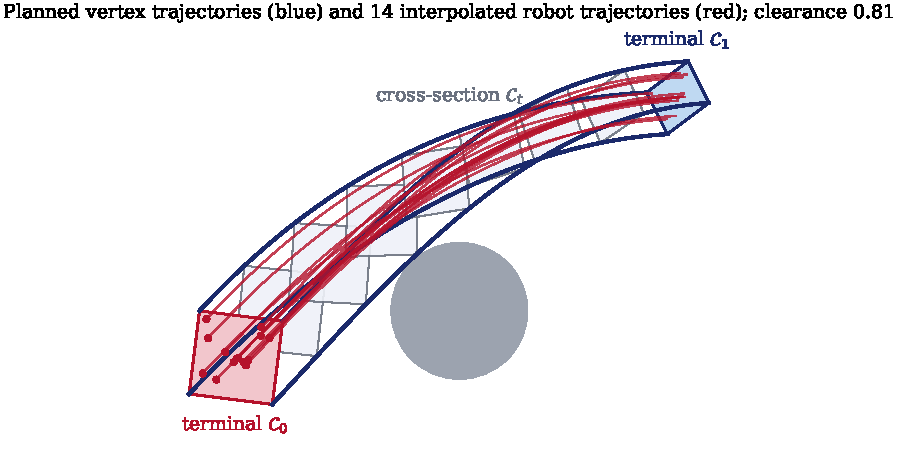
\includegraphics[width=0.9\linewidth]{virtual-tube}
  \caption{A linear virtual tube with convex-hull terminals. Only the four vertex
           trajectories (blue) are planned; each robot starts at a convex
           combination of the vertices of $\mathcal{C}_0$ and follows the same
           combination of the vertex trajectories (red).}
  \label{fig:virtual-tube}
\end{figure}

\Cref{fig:virtual-tube} shows the geometric structure of a virtual tube. The
start region (terminal $\mathcal{C}_0$) and the goal region (terminal
$\mathcal{C}_1$) are the entry and exit sets of the swarm. Each robot moves
along a trajectory $\mathbf{h}\bigl((\mathbf{q}_0, \mathbf{q}_m), t\bigr)$ from
its start point $\mathbf{q}_0$ to its exit point $\mathbf{q}_m$, and the shaded
polygons are cross-sections $\mathcal{C}_t$ of the tube at several times. Because
every cross-section is convex and the tube avoids the obstacle, any robot that
starts inside $\mathcal{C}_0$ stays inside the tube and away from the obstacle,
and many robots can pass through it at the same time.

\subsection{The Concept of Virtual Tubes}

A virtual tube is a bounded region of free space that connects the start and goal
regions and is constructed to maximize the safety margin and maintain acceptable
cross sections along the path, so that many robots can pass through
simultaneously without deadlock. Once the tube is available, path planning
reduces to assigning each robot a feasible path that stays inside the corridor
and respects minimum distances, which greatly simplifies downstream control and
coordination \cite{mao2023optimal}.

\subsubsection{Definition and Components}

Formally, a virtual tube $T$ in an $n$-dimensional configuration space is a
4-tuple $(\mathcal{C}_0, \mathcal{C}_1, f, h)$ \cite{mao2023optimal}. The
terminals $\mathcal{C}_0$ and $\mathcal{C}_1$ are disjoint, bounded, convex sets
(convexity makes them simply connected); $f : \mathcal{C}_0 \to \mathcal{C}_1$ is
a diffeomorphism that pairs every start point with an exit point, producing the
ordered pairs $\mathcal{P} = \{(\mathbf{q}_0, \mathbf{q}_m) : \mathbf{q}_0 \in
\mathcal{C}_0,\ \mathbf{q}_m = f(\mathbf{q}_0)\}$; and
$h : \mathcal{P} \times [0,1] \to T$ is a smooth map that generates the
trajectory of each pair. The cross-section at time $t$ is
$\mathcal{C}_t = \{h((\mathbf{q}_0,\mathbf{q}_m), t) : (\mathbf{q}_0,\mathbf{q}_m)
\in \mathcal{P}\}$, and every cross-section is simply connected and varies
continuously. Earlier definitions built around a generator curve are special
cases. The space is $n$-dimensional rather than three-dimensional because the
motion of a rigid robot in 3-D is described by a six-dimensional manifold.
In words:
\begin{itemize}
  \item \lead{Terminals} The start and goal regions, which delimit the entry and
        exit sets of the swarm and are chosen as simple bounded regions so that
        they can be filled without conflicts.
  \item \lead{Mapping and assignment} Establishing entry--exit pairs between the
        entry points in the start region and the exit points in the goal region,
        which are often induced by a global planner that enumerates the homotopy
        classes around the obstacles.
  \item \lead{Paths and cross sections} A family of feasible paths inside the
        corridor and their instantaneous cross sections, designed to remain
        connected and sufficiently wide to prevent congestion and maintain
        separation.
\end{itemize}

\subsubsection{Linear Tubes and the Interpolation Idea}

In practice, many deployments use linear or piecewise-linear centerlines and
polyhedral cross sections, so that the interior paths of the agents can be built
from convex combinations of, or simple interpolations between, boundary
references while preserving feasibility and spacing. A tube is \emph{linear} when
both $f$ and $h$ are linear maps; in the most useful case, the linear virtual
tube with convex-hull terminals, $\mathcal{C}_0$ and $\mathcal{C}_1$ are convex
hulls (polyhedra) of finite vertex sets and $f$ maps vertex to vertex. Under the
conditions given in \cite{mao2023optimal}, every trajectory inside such a tube
that is a convex combination of optimal vertex trajectories is itself optimal.
The planner therefore solves only a few boundary problems and obtains every other
trajectory by interpolation, which reduces the cost from
$O\bigl(k(n_t,\varepsilon)\,n_t^{2}\bigr)$--$O\bigl(k(n_t,\varepsilon)\,n_t^{3}\bigr)$
per robot to $O(n_t)$ and makes the method suitable for large swarms
\cite{mao2023optimal}.

\subsection{Optimal Virtual Tube Planning}

OVTP selects safety-margin-aware corridors and a small set of reference paths,
and it then efficiently generates the many robot paths so as to minimize
congestion and computation while guaranteeing obstacle avoidance. This approach
amortizes the heavy global search over the group and replaces independent global
planning for each robot with a lightweight synthesis inside the tube \cite{mao2023optimal}.

\subsubsection{Hierarchical Planning with MPC Tracking}

A practical architecture computes the tube(s) and the reference paths centrally
and then deploys distributed controllers (e.g., MPC) on each robot to track its
assigned path and to enforce the tube and inter-robot constraints in real time
\cite{mao2023optimal}.

MPC naturally handles receding-horizon collision avoidance and adherence to the
boundaries through inequality constraints: the position of a robot is
constrained to the interior of the tube, or to a band near its boundary for
robots on the boundary. This gives formation-like cohesion and robust tracking,
and in simulations and experiments the combination outperformed formation
control and plain predictive control in obstacle-dense environments
\cite{mao2023optimal}.

\subsubsection{Objectives: Computation, Volume, and Energy}

\begin{itemize}
  \item \lead{Computation} By reusing the same corridor and a small set of
        references, the synthesis for each agent reduces to interpolation or
        projection and local smoothing, which lowers the complexity compared with
        complete replanning for every robot.
  \item \lead{Minimum cross-sectional volume} Corridors are selected to preserve a
        sufficient cross-sectional ``capacity'' at bottlenecks; margin-aware
        backbones such as the GVD or homotopic paths preserve a safe tube
        thickness. Tube-\RRTstar{} measures this by the minimum gap volume, the
        volume of the smallest gap the path passes through \cite{mao2024tube}.
  \item \lead{Energy} Smooth curvature and non-crossing assignments reduce the
        demands for acceleration and turning and improve energy efficiency while
        maintaining throughput; choosing $f$ so that trajectories do not
        intersect serves the same purpose \cite{mao2023optimal}.
\end{itemize}

\subsubsection{Tube Networks for Complex Obstacles}

When a single corridor is insufficient, multiple tubes form a network that splits
the swarm into parallel routes around large obstacles and merges it again
downstream, thereby reducing congestion and delay. Designing consistent
assignments across the branches and avoiding internal crossings are essential for
preserving the distinction between the boundary and the interior and for
supporting safe merging behaviors; how to build such networks is still an open
question \cite{mao2023optimal}.

%-----------------------------------------------------------------------------
\section{Summary}\label{sec:ch3-summary}

This chapter reviewed and analyzed a wide range of path planning methods for
swarm robotic systems. These methods were divided into three broad
categories---deterministic, AI-based, and hybrid---each with its own distinctive
characteristics and applications. Based on this analysis, the following
conclusions can be drawn:
\begin{enumerate}
  \item \lead{Deterministic methods} Classical algorithms such as \Astar{} and
        cell decomposition perform reliably in static, known environments and
        guarantee that a path will be found. However, as discussed in
        \cref{sec:global-local}, these methods suffer from problems such as high
        computational cost and inflexibility in dynamic and complex environments.
        Sampling-based algorithms such as \RRTstar{} have partially addressed
        these challenges in high-dimensional spaces by striking a balance between
        speed and optimality.
  \item \lead{AI-based methods} This category---especially bio-inspired algorithms
        such as PSO and ACO---is highly compatible with swarm robotics owing to
        its distributed nature. The review showed that PSO, through its velocity
        and position update formula (\cref{eq:pso}), enables fast convergence in
        dynamic environments and, in most complex scenarios, succeeds in finding
        the shortest path and the minimum time simultaneously. In addition,
        reinforcement learning methods (RL and deep Q-learning) have shown great
        potential for navigation in unknown environments without a prior map.
  \item \lead{Hybrid methods} Hybrid approaches, which account for about 25\% of
        recent research, integrate the strengths of deterministic and intelligent
        methods in an attempt to overcome the limitations that each has on its
        own.
\end{enumerate}

Finally, the choice of an appropriate method depends strongly on the type of
mission (static or dynamic), on hardware limitations (processing and
communication), and on system priorities (time versus energy consumption). For
real-time applications and dynamic environments, hybrid and AI-based methods
(especially PSO and \RRTstar) are considered the superior options.

%=============================================================================
\chapter{Challenges and Applications of Path Planning in Swarm Robots}\label{chap:challenges}
%=============================================================================

This chapter examines the complexities of deploying swarm robots, particularly
with respect to their navigation and coordination, and then reviews the main
domains in which swarms are being applied.

%-----------------------------------------------------------------------------
\section{Challenges in Dynamic and Complex Environments}\label{sec:dynamic-challenges}

With complex obstacles, large search spaces, and unpredictable changes, the
difficulty of path planning increases dramatically. In multi-robot systems,
simultaneous operation creates a risk of collisions between the robots and with
obstacles, which can lead to equipment damage, delays, or mission failure;
collision avoidance therefore becomes a critical challenge
\cite{oh2025survey,lin2022review}.

\subsection{Obstacle Avoidance and Collision Resolution}

In the swarm robotics community, obstacle avoidance is regarded as a basic and
important task. It refers to the ability of robots to move around obstacles
without colliding with them, mimicking the maneuverability observed in
biological swarms \cite{tan2016handbook}.

\subsubsection{Collision Avoidance Strategies in Dynamic Environments}

In a dynamic environment, the ability of the planning algorithm to adjust the
path in real time to accommodate moving obstacles, changes in the layout of the
environment, or relocated targets is essential. The challenge intensifies when
the moving obstacles have unknown headings, which makes accurate prediction of
potential blocking points difficult \cite{li2021rrt}.

The strategies used for collision avoidance in dynamic multi-robot systems
typically emphasize real-time adaptability and computational efficiency:
\begin{itemize}
  \item \lead{Decentralization} The strategies are generally distributed and
        based on local information and communication constraints, which
        contributes to robustness and adaptability \cite{oh2025survey}.
  \item \lead{Real-time replanning} The rapidly-exploring random tree (RRT)
        algorithm and its variants have been adapted to operate in real time in
        dynamic environments. One strategy grafts new waypoints onto the
        existing path based on local obstacle avoidance; by avoiding the
        recomputation of the entire original path when an obstacle is detected,
        it greatly reduces the computation time and reaches the corrected path
        with a relatively short deviation from the initial one \cite{li2021rrt}.
  \item \lead{Learning-based methods} Deep reinforcement learning (DRL) methods
        are increasingly preferred over classical methods because they handle
        collision avoidance in high-dimensional spaces without requiring the
        robots' kinematics or a global map \cite{zhang2025deep,huttenrauch2019deep}.
\end{itemize}

\subsubsection{Potential Force Methods for Collision Avoidance}

The artificial potential field, introduced by Khatib in 1986, is the classical
basis of real-time collision avoidance: the goal attracts, the obstacles repel,
and the robot moves under the resulting force \cite{khatib1986real}.
\begin{itemize}
  \item \lead{Avoidance mechanism} Repulsion from an obstacle has been likened to
        the mechanism of an atomic nucleus: the obstacle generates a virtual
        repulsive force, and the robots maneuver around it like electrons
        \cite{tan2016handbook}.
  \item \lead{Priority and guarantee} The collision avoidance mechanism must take
        precedence over all other actions \cite{sahin2007swarm}. With properly
        defined potential functions, a mathematical guarantee can be given that
        no collision will occur, provided that the repulsive force becomes
        unbounded as the distance tends to zero \cite{khatib1986real}.
  \item \lead{Swarm coordination} Potential functions are used to guide swarms
        and to modify the desired positions of the robots so that they circumvent
        obstacles; shape controllers combine several potential forces to reach a
        formation while avoiding collisions \cite{tan2016handbook}.
\end{itemize}

\subsubsection{Obstacle Enlargement and Robot Shrinking}

A simplifying deterministic technique in path planning is to adjust the effective
size of the obstacles or of the robot in order to simplify collision checking
\cite{lin2022review}.
\begin{itemize}
  \item \lead{Principle} This mechanism achieves collision avoidance by
        effectively enlarging the obstacles and shrinking the moving body to a
        point mass.
  \item \lead{Application} In constrained optimization formulations (such as
        global path planning in a static environment), the radii of convex
        polygonal and circular obstacles are increased in proportion to the
        physical dimensions of the robot. The robot is thus modeled as a
        particle that remains collision-free as long as it stays outside the
        boundary of the enlarged obstacle \cite{tan2016handbook}.
\end{itemize}

\subsubsection{Optimal Reciprocal Collision Avoidance (ORCA)}

ORCA is a powerful and widely used variant of the reciprocal velocity obstacle
(RVO) methods for collision-free navigation \cite{vandenberg2011reciprocal}.
\begin{itemize}
  \item \lead{Mechanism} Assuming that the velocities of the neighbors are known
        and exchanged, ORCA selects a collision-free velocity for each agent in
        real time by solving a small linear program over half-plane constraints.
  \item \lead{Efficiency} For an agent with $k$ neighbors, ORCA takes $O(k)$ time
        \cite{zhou2017fast}.
  \item \lead{Comparison with Voronoi-based methods} ORCA is often compared with
        the buffered Voronoi cell (BVC) method, which has the same complexity and
        similar empirical performance. The key difference lies in the exchange of
        information: ORCA relies on communication to share positions and
        velocities, whereas BVC needs only the sensed relative positions to
        guarantee avoidance \cite{zhou2017fast}.
\end{itemize}

\subsection{Unknown and Dynamic Environments}

The transition from controlled laboratory settings to real-world applications
requires handling environments whose information is incomplete or that change
continuously. Under these conditions, swarm path planning must address real-time
search, robust coordination, and dynamic target seeking.

\subsubsection{Search-and-Rescue Missions in Hazardous Conditions}

Search-and-rescue (SaR) operations are a key target for swarm robotics, because
these scenarios are inherently complex and hostile and challenge the application
of traditional multi-robot systems \cite{tan2016handbook}.
\begin{itemize}
  \item \lead{Characteristics of SaR environments} Large extents, from hundreds
        of square meters to hectares; strong dynamics caused by the agents
        themselves and by external events such as collapses, fires, floods, and
        earthquakes; and harsh conditions, including abrasive dust, water,
        chemicals, and numerous obstacles that damage the hardware and disrupt
        communication \cite{tan2016handbook}.
  \item \lead{Advantages of swarms} Robustness to the failure of units,
        scalability, and reliance on self-organization improve the emergency
        response through damage assessment, resource management, and movement
        through complex environments to find and assist survivors. Examples
        include aquatic drones searching flooded areas and nano-robots proposed
        for cleaning up hazardous materials \cite{bhowmick2024bio}.
\end{itemize}

\subsubsection{Adapting to Moving Targets and Changing Conditions}

An important challenge arises when the targets, the obstacles, or the terrain are
not fixed but change dynamically and unpredictably \cite{tan2016handbook,lin2022review}.
\begin{itemize}
  \item \lead{Handling dynamic changes} Swarm systems must react and adapt in real
        time to changes in the terrain, in environmental conditions (such as
        weather and currents), or to unexpected obstacles, for example shifting
        debris after a disaster \cite{bhowmick2024bio}.
  \item \lead{Moving target tracking (MTT)} In an environment full of obstacles,
        the swarm must simultaneously move as a flock, avoid the obstacles, and
        maintain enough collective coverage that a randomly moving target never
        leaves its sight; this problem is relevant to escorting, monitoring, and
        group transport \cite{tan2016handbook}.
  \item \lead{Difficulty of prediction} In environments with moving obstacles
        whose headings are unknown, determining the potential blocking points is
        difficult \cite{li2021rrt}.
  \item \lead{Adaptive algorithms} Continuous motion and adaptation call for
        algorithms with predictive capabilities, such as bio-inspired optimizers
        that model warning behavior for cooperative planning in dynamic
        environments \cite{lin2022review}.
\end{itemize}

\subsubsection{Real-Time Path Planning for Multi-Robot Systems}

In dynamic, unknown, or partially known environments, computing an optimal global
path is often prohibitively expensive, so the focus shifts to efficient real-time
local strategies for planning and replanning:
\begin{itemize}
  \item \lead{Dynamic grid search (\Dstar{} and \Dstar{} Lite)} \Dstar{} extends
        \Astar{} to changing maps: by updating the weights of the edges affected
        by newly observed obstacles, it repairs only the necessary parts of the
        path instead of replanning completely \cite{stentz1994optimal,koenig2002d}.
  \item \lead{Time rolling windows} Combined with local optimizers such as ABC,
        PSO, or the fireworks algorithm, a rolling time window in which each
        robot perceives and predicts its surroundings replaces costly global
        planning in dynamic and unknown environments \cite{tan2016handbook}.
  \item \lead{RRT-based real-time replanning} The RRT family is well suited to
        dynamic environments because it accounts for the dynamic constraints of
        the robot; grafting adds new waypoints to the existing path, which
        reduces the computational load of a complete recomputation
        \cite{li2021rrt}.
  \item \lead{Artificial potential field} The APF is valuable for rapid path
        adjustment because of its fast reaction to nearby obstacles, but it is of
        limited use in highly complex environments because of the risk of getting
        trapped in local minima (\cref{fig:apf}) \cite{zhang2023multi}.
\end{itemize}

\subsection{Adaptation and Real-Time Replanning}

The growing demand for deploying multi-robot systems in complex real-world
scenarios has made it necessary to move from offline, static planning to
strategies for real-time adaptation and rapid replanning.

\subsubsection{Dynamic Multi-Robot Systems and Environmental Changes}

Path planning in dynamic environments is multifaceted: the environment changes
because of external factors, moving targets, or the actions of the robots
themselves \cite{tan2016handbook}.
\begin{itemize}
  \item \lead{Need for real-time reaction} Algorithms must adapt quickly to
        changes; traditional deterministic methods often fail to adapt rapidly to
        unexpected obstacles and are computationally expensive \cite{abujabal2024path}.
  \item \lead{Environmental instability} In applications such as SaR after
        natural disasters, the environment can change rapidly (falling debris,
        weather conditions, unexpected events), and the algorithms must allow the
        behavior and the flight or motion patterns to be changed immediately
        \cite{bhowmick2024bio}.
  \item \lead{Adaptability and flexibility} The swarm must be flexible enough to
        cope with various tasks and situations and to adjust its paths as water
        or air currents change or as obstacles appear \cite{tan2013research}.
  \item \lead{Complexity of distributed control} Controlling groups of simple,
        reactive robots in a distributed structure is difficult, because the
        desired macroscopic behaviors emerge only from local interactions, and
        path planning must respond to continuously changing scenarios without
        relying on a limited set of predefined conditions
        \cite{brambilla2013swarm}.
\end{itemize}
This demand for adaptability has pushed research toward learning-based methods,
which let robots improve their strategies from experience
\cite{kuckling2023recent}.

\subsubsection{RRT-Based Algorithms for Replanning}

The RRT family and its variants are suitable for dynamic environments because of
their ability to generate feasible paths and to incorporate the dynamic
constraints of the robot directly \cite{li2021rrt}.
\begin{itemize}
  \item \lead{RRT-Connect and optimality} RRT and its enhanced versions, such as
        RRT-Connect and \RRTstar, have been explored in dynamic environments;
        although \RRTstar{} provides asymptotic optimality, it can be
        computationally expensive \cite{chen2025survey}.
  \item \lead{Grafting for real-time efficiency} Grafting adds new points based on
        local avoidance and nonholonomic constraints, generating a new point when
        a potential collision is detected in the next sampling step. Instead of
        recomputing the whole tree, only a short detour results \cite{li2021rrt}.
\end{itemize}

Dynamic variants include \cite{chen2025survey}:
\begin{itemize}
  \item \lead{DRRT} Provides fast, feasible, but sub-optimal paths by pruning and
        regrowing the affected parts of the tree.
  \item \lead{\RRTstar FND} Achieves asymptotic optimality through repeated
        updates in a dynamic environment, albeit at a high computational cost.
  \item \lead{RT-\RRTstar} Retains the full tree structure without pruning, which
        enables fast queries for multiple goals and rapid rewiring of the path in
        response to dynamic obstacles and changing goals.
\end{itemize}

%-----------------------------------------------------------------------------
\section{Scalability and Robustness}\label{sec:scalability}

Scalability and robustness are common and essential properties of swarm systems
that enable them to operate effectively in complex real-world scenarios.
Robustness refers to the ability of the system to function normally despite
disturbances or individual failures, whereas scalability refers to the ability
to maintain effective operation across different population sizes
\cite{dias2021swarm,brambilla2013swarm}.

\subsection{Scalability in Swarm Systems}

Scalability is both a critical challenge and a defining characteristic of swarm
robotics: the system must work with arbitrary population sizes, from a few units
to potentially thousands. Since the control method is usually identical for every
member of the swarm, the system is designed to be highly scalable
\cite{dias2021swarm,tan2013research}.

\subsubsection{Maintaining Performance as the Number of Robots Increases}

Scalability is the capacity of the system to adjust the number of robots flexibly
without a noticeable change in its overall functionality or an excessive drop in
efficiency or reliability \cite{dias2021swarm,tan2013research}.
\begin{itemize}
  \item \lead{Design principle} Scalability stems from decentralization and from
        predominantly local interactions. Methods that rely on global
        broadcasting or on monitoring large parts of the swarm are avoided in
        order to preserve scalability, and local sensing and communication
        facilitate this property \cite{brambilla2013swarm}.
  \item \lead{Ideal versus actual performance} In the ideal case, a
        super-scalable system performs almost independently of the number of
        robots; in a merely scalable system, the loss of efficiency as units are
        added is small; in an unscalable one, population growth causes severe
        degradation or failure \cite{tan2013research}.
  \item \lead{Cognitive complexity} For independently operated robots, the
        operator's workload grows as $O(n)$, whereas with proper distributed
        coordination, swarm control can bring it down to $O(1)$
        \cite{hart2004reducing,kolling2016human}.
  \item \lead{Effect on tasks} Adding or removing members should not jeopardize
        the completion of the mission, and implicit reallocation of tasks should
        occur without external intervention \cite{tan2013research}.
  \item \lead{Challenges} As the number of robots increases, maintaining
        productivity becomes harder and requires mechanisms such as control
        hierarchies and clustering to manage the communication and processing
        load and to prevent bottlenecks \cite{bhowmick2024bio}.
\end{itemize}

\subsubsection{Simulation of Large-Scale Swarms}

Because swarm algorithms are meant to scale to populations that are hard to
build physically, simulating hundreds or thousands of robots is a vital part of
research, and modeling and simulation are the necessary tools for this purpose
\cite{dias2021swarm,hamann2018swarm}. Notable simulators and platforms include:
\begin{itemize}
  \item \lead{ARGoS} A modular simulator that can run several physics engines in
        parallel; it can simulate 10,000 e-pucks in 60\% of the time the real
        experiment would take \cite{dias2021swarm,pinciroli2012argos}.
  \item \lead{Player/Stage/Gazebo} An open-source framework with multi-robot
        capabilities; for 2-D swarm behaviors, its run time scales approximately
        linearly up to at least 100,000 simple robots \cite{tan2016handbook}.
  \item \lead{Kilobot} A low-cost, small physical platform built to test collective
        algorithms with hundreds to thousands of robots; a thousand Kilobots have
        self-assembled into programmed shapes \cite{rubenstein2014programmable}.
\end{itemize}

\subsubsection{Exponential Growth of States in Modular Robotics}

Although scalability usually refers to functioning independently of the size of
the population, in modular robotic systems the complexity of a configuration
space with many degrees of freedom poses a distinct challenge \cite{yim2007modular}.
\begin{itemize}
  \item \lead{Modular systems} Self-reconfigurable systems such as M-TRAN, ATRON,
        and PolyBot are designed to build and form complex structures.
  \item \lead{State explosion} The number of possible configurations grows
        exponentially with the number of modules, which makes centralized
        planning and control difficult and reinforces the need for robust local
        rules.
\end{itemize}
If each of $n$ modules can be in one of $k$ states, the number of combinations is
\begin{equation}
  S = k^{n},
  \label{eq:state-explosion}
\end{equation}
before connectivity constraints are taken into account. Chain-type modular robots
are particularly versatile, but managing this explosion remains a key
computational obstacle \cite{yim2007modular}.

\subsection{Robustness and Fault Tolerance}

Robustness and fault tolerance are fundamental properties of swarm robotic
systems; they mean maintaining operation and a desired level of performance in
the face of internal failures or external disturbances
\cite{dias2021swarm,brambilla2013swarm}.

\subsubsection{Robustness to Failures of Individual Robots}

Robustness to individual failures stems mainly from redundancy and from the
absence of a centralized point of control \cite{dias2021swarm,tan2013research}.
\begin{itemize}
  \item \lead{Massive redundancy} The large number of robots provides critical
        redundancy for safety and fault tolerance, and the loss of one robot can
        be compensated for by the others.
  \item \lead{Distributed control} The absence of a single point of failure means
        that the failure of one node or part does not disable the whole system.
  \item \lead{Performance preservation} The design treats individuals as
        dispensable, so a swarm can lose a considerable share of its robots
        before the mission has to be abandoned, albeit with reduced capability
        \cite{tan2016handbook}.
  \item \lead{Fault detection} The natural redundancy of the swarm can be used to
        detect faulty robots; for example, robots that flash in synchrony, like
        fireflies, can flag a peer that falls out of step as faulty
        \cite{brambilla2013swarm}.
\end{itemize}

\subsubsection{Fault Tolerance and Redundancy in Communication}

Ensuring the robustness of communication in dynamic and crowded environments is
challenging and requires special mechanisms to cope with failures, interference,
and delays \cite{bhowmick2024bio}.
\begin{itemize}
  \item \lead{Redundant communication paths} Establishing alternative paths helps
        maintain the robustness of the network if one path is broken.
  \item \lead{Distributed nodes and reconfiguration} Distributing communication
        tasks among several robots and reconfiguring the network dynamically
        adapt it to changing conditions and reduce the impact of faults.
  \item \lead{Information redundancy} Replicating critical information across
        several robots preserves its availability in the face of communication
        problems.
  \item \lead{MANETs and multi-connectivity} In missions such as SaR, the robots
        must maintain a mobile ad hoc network (MANET) without pre-existing
        infrastructure, using attractive forces and redundancy to stay
        connected. The notion of $k$-connectivity generalizes bi-connectivity:
        the network stays connected as long as fewer than $k$ nodes fail, that
        is, when its vertex connectivity satisfies $\kappa(G) \ge k$
        \cite{tan2016handbook}.
\end{itemize}

%-----------------------------------------------------------------------------
\section{Task Allocation and Coordination}\label{sec:task-allocation}

Multi-robot task allocation (MRTA) is the problem of assigning tasks to
individual robots so as to maximize the expected performance of the overall
system, and it is usually treated as an instance of the optimal assignment
problem. In swarm robotics, this coordination is vital for distributing the work
and ensuring that collective goals are achieved efficiently under decentralized
control \cite{brambilla2013swarm,yan2013survey}.

\subsection{Dynamic Task Allocation}

Dynamic task allocation refers to strategies in which the matching between tasks
and robots is computed repeatedly over time, so that the robot team adapts to
changing conditions, tasks, or environments; online allocation can react to such
changes, whereas simple offline methods cannot \cite{yan2013survey}.

\subsubsection{Efficient Achievement of Collective Goals}

Achieving collective goals requires a distribution of tasks that takes into
account the capabilities of the robots, their workload, and the environmental
constraints, so as to maximize the performance of the whole swarm and minimize
unnecessary redundancy \cite{brambilla2013swarm}.
\begin{itemize}
  \item \lead{Task partitioning} Decomposing tasks greatly improves efficiency.
        In sequential tasks, robots can measure how long they wait for another
        subtask to be completed and use this local cue to decide whether to
        partition the work, so that interdependent subtasks run concurrently and
        interference is reduced \cite{brambilla2013swarm}.
  \item \lead{Decentralized decision-making} For scalability and robustness, each
        robot selects and prioritizes tasks based on its own state, its sensor
        data, and the mission goals \cite{bhowmick2024bio}.
  \item \lead{Optimization objectives} Criteria such as minimizing the completion
        time, maximizing resource utilization, or balancing the load among robots
        are used; maximizing collective utility when group dynamics affect
        performance is in general NP-hard \cite{yan2013survey}. Consensus-based
        allocation has been used to make the assignment both fast and
        energy-efficient \cite{mahato2023consensus}.
\end{itemize}

\subsubsection{Heuristic Algorithms for Distributed Task Selection}

The distributed task selection problem in a swarm is NP-complete, so
polynomial-time heuristics are used to obtain good-enough solutions
\cite{sahin2007swarm}.
\begin{itemize}
  \item \lead{Model and objective} The mechanism tries to assign the desired number
        of swarm units to each task while reducing inter-task delays and
        communication overhead.
  \item \lead{Performance of the heuristics} Heuristics in which each unit
        considers both the effect of the other units on the tasks and its own
        relative position give better task processing and a better distribution
        of units over the tasks.
  \item \lead{Communication constraints} These approaches work without a central
        location or shared memory, using only distributed communication.
\end{itemize}
Auction- and market-based methods are the main alternatives to such heuristics
\cite{yan2013survey}.

\subsubsection{Task Scheduling in Layered Architectures}

In hierarchical or layered architectures, a scheduling layer manages the overall
flow of the mission: at each instant, it selects the subset of tasks that should
run concurrently, elects the robot that coordinates them, and decides how many
tasks to request from each deployment point. A global planner may propose the
allocation, which the scheduling layer then distributes to the swarm; the point
is to approximate a good strategy for the robots' navigation controllers at a
small computational cost while respecting the timing and ordering constraints of
the tasks \cite{yan2013survey,liu2019distributed}.

\subsection{Cooperative Control and Manipulation}

Cooperative control is the problem of steering a multi-agent system toward a
common goal (exploration, search, rescue, etc.); integrating multiple robots
increases capacity, flexibility, and efficiency \cite{yan2013survey}.

\subsubsection{Multi-Robot Teamwork Strategies}

For cohesive and efficient operation, multi-robot systems require coordination
strategies that ensure inter-robot communication, effective task allocation, and
conflict resolution \cite{yan2013survey}.
\begin{itemize}
  \item \lead{Decentralized coordination} For scalability and robustness,
        coordination must be decentralized and based on local interactions and
        simple rules, so that global behaviors emerge from local interactions
        \cite{brambilla2013swarm}.
  \item \lead{Implicit versus explicit} Cooperation can emerge implicitly from the
        autonomous decisions of individuals or be supported by explicit
        communication (subject to bandwidth constraints) to improve information
        exchange and motion synchronization.
  \item \lead{Behavioral approaches} Behavior-based formation control and
        distributed control manage interactions and resolve conflicts with local
        information; a controller based on several potential forces can steer
        the robots toward the desired shape and prevent collisions
        \cite{tan2016handbook}.
  \item \lead{Hierarchical architectures} Hybrid-HASP
        (\cref{sec:control-architectures}) combines competitive and cooperative
        mechanisms to select and combine elementary behaviors, and it supports
        cooperation through implicit communication with simple attractive and
        repulsive signals \cite{tan2016handbook}.
\end{itemize}

\subsubsection{Cooperative Grasping and Object Transport}

Cooperative transport and manipulation (e.g., box pushing) is a common benchmark
and usually involves objects that a single robot cannot handle
\cite{bonabeau1999swarm,brambilla2013swarm}.
\begin{itemize}
  \item \lead{Physical requirements} A physical connection (self-assembly) is
        necessary to cross large gaps or to perform complex transport;
        cooperative grasping requires communication and docking before
        execution.
  \item \lead{The Swarm-bot project} This project showed that autonomous agents
        relying solely on local information can cooperatively transport heavy
        objects that a single robot cannot move; the aggregation of s-bots into a
        formation plays a key role \cite{mondada2003swarmbot,gross2006object}.
  \item \lead{Coordinated motion} In cooperative transport, the robots must share
        information about the object and the destination, agree on a common
        direction, and then move together; Hybrid-HASP has been used to
        coordinate box pushing \cite{tan2016handbook}.
\end{itemize}

\subsubsection{Consensus, Tracking, and Containment}

Path planning for cooperative swarms must address the fundamental objectives of
consensus, maintenance of relative positions or formation (tracking), and
containment \cite{li2014cooperative}.
\begin{itemize}
  \item \lead{Consensus control} The group must reach agreement on the variables
        of interest; consensus algorithms, close relatives of distributed linear
        algorithms, typically move each agent toward the average of the values it
        receives \cite{bullo2009distributed}.
  \item \lead{Tracking and formation control} Formation is a key application of
        cooperative control whose aim is to achieve a fixed geometric pattern;
        leader--follower and flocking approaches are used, the latter with
        collision avoidance, velocity matching, and flock centering
        \cite{reynolds1987flocks,li2014cooperative}. A simulation of
        leader--follower tracking is shown in \cref{fig:leader-follower}.
  \item \lead{Containment and region control} In region control, the group is kept
        within a predefined region using constraint functions, and in multilevel
        designs, the robots converge to the region and form the shape level by
        level \cite{tan2016handbook}.
\end{itemize}
With several leaders, containment requires every follower to stay in the convex
hull spanned by the leaders,
\begin{equation}
  x_i(t) \in \operatorname{conv}\bigl\{x_j(t) : j \in \mathcal{L}\bigr\},
  \label{eq:containment}
\end{equation}
where $\mathcal{L}$ is the set of leaders \cite{li2014cooperative}.

\begin{figure}[htbp]
  \centering
  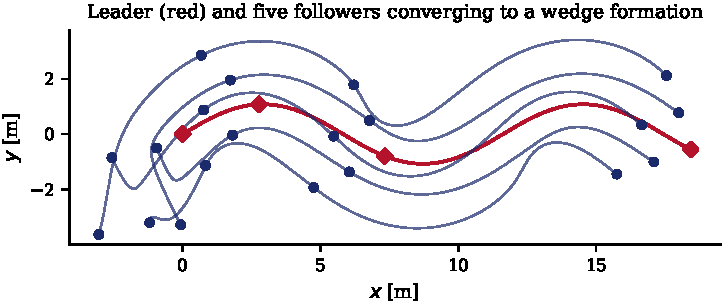
\includegraphics[width=0.85\linewidth]{leader-follower}
  \caption{Leader--follower formation tracking: five followers start from random
           positions and converge, through local consensus on their formation
           errors, to a wedge around the leader (markers every few seconds).}
  \label{fig:leader-follower}
\end{figure}

%-----------------------------------------------------------------------------
\section{Real-World Applications of Swarm Robotics}\label{sec:applications}

The ultimate goal of swarm robotics research is to deploy these systems in
real-world scenarios, especially where the tasks are too hazardous, complex, or
large-scale for individual robots or human teams. Although swarm robotics has
long been confined to academia, the field is moving toward practical
applications \cite{kegeleirs2025towards,shahzad2023review}. Examples are compiled
in \cref{tab:applications} and discussed below.

\begin{table}[htbp]
  \centering
  \caption{Examples of real-world applications of swarm robotics.}
  \label{tab:applications}
  \small
  \rowcolors{2}{lightbg}{white}
  \begin{tabularx}{\linewidth}{@{}>{\bfseries\raggedright\arraybackslash}p{0.18\linewidth}LLL@{}}
    \toprule
    \rowcolor{white}
    Application domain & \textbf{Specific tasks and missions}
      & \textbf{Example platforms or projects} & \textbf{Key advantages and methods} \\
    \midrule
    Agriculture & Precision weeding, crop monitoring
      & LettuceBot, senseFly \cite{bhowmick2024bio}
      & Less herbicide through machine vision; continuous monitoring \\
    Search and rescue & Locating survivors in rubble, flood response
      & RoboBees, AquaDrones \cite{bhowmick2024bio}
      & Rapid area coverage; operation without GPS or infrastructure \\
    Construction & Bricklaying, site inspection
      & Skycatch \cite{bhowmick2024bio}
      & Parallel work and faster construction \\
    Environmental monitoring & Water quality, marine pollution
      & microUSV, CoCoRo \cite{dias2021swarm,shahzad2023review}
      & Distributed sensing and collective mapping \\
    Warehousing and logistics & Goods handling in warehouses
      & Kiva \cite{shahzad2023review}
      & Decentralized path coordination in crowded spaces \\
    Space exploration & Resource prospecting, in-space assembly
      & Swarmies, Marsbees \cite{shahzad2023review}
      & Redundancy and fault tolerance far from help \\
    \bottomrule
  \end{tabularx}
\end{table}

\subsection{Search and Rescue}

\subsubsection{Exploring Hazardous Environments}

Disaster sites are hostile, dynamic, and large, with dust, water, chemicals, and
debris, and these conditions cannot be handled by simply adapting traditional
planning and control \cite{tan2016handbook}. Swarms survive such conditions
through redundancy, and they can map collapsed structures and identify hazards,
locate trapped survivors by body heat, heartbeat, or sound, and track chemical or
radiation leaks \cite{bhowmick2024bio}. Proposed and demonstrated examples
include insect-sized flying robots (RoboBees) for searching collapsed buildings,
aquatic drones (AquaDrones) and amphibious robots for floods, and swarms for
demining \cite{bhowmick2024bio}.

\subsubsection{Initial Deployment and Communication in Faulty Environments}

Two open problems in real SaR missions are the initial deployment of the robots
and the integrity of their network \cite{tan2016handbook}. The initial placement
strongly affects the efficiency of the search; options include random
deployment, contextual deployment that uses map or network-quality information,
and marsupial deployment, in which a larger robot carries and releases smaller
ones. Communication is hard because obstacles are everywhere, the topology of the
MANET keeps changing, and low batteries make nodes fail. Simple range-based rules
are unreliable, so approaches refresh connectivity tables continuously and limit
the robots' motion to keep multi-hop routes of sufficient quality. Virtual
attractive forces based on signal strength keep a robot close to its neighbors
while repulsive forces prevent collisions, and redundancy lets the remaining
robots fill the gap left by one that loses contact \cite{tan2016handbook}.

\subsection{Environmental Monitoring and Mapping}

\subsubsection{Mapping Scalar Fields and Marine Environments}

A common mission is to map an unknown scalar field, such as temperature,
salinity, or pollutant concentration, over a large area, which suits mobile robot
networks. In one cooperative scheme, each robot runs two distributed consensus
filters: a weighted-average consensus filter estimates the field value, an
average consensus filter estimates the confidence of that estimate, and the map
is refined with a weighted-average protocol as the robots move
\cite{tan2016handbook}. At sea, the CoCoRo project used 41 heterogeneous
underwater vehicles, communicating through electric fields and sonar, for
environmental monitoring, while the Platypus system uses swarms of surface
vessels to map water quality and stratify salinity and oxygen levels
\cite{shahzad2023review}.

\subsubsection{Chemical Plume Tracing and Source Localization}

Chemical plume tracing (CPT) steers robots, instead of people, toward the source
of toxic gas leaks, fires, or explosives. It is hard in natural environments
because the source strength and the advection distance are unknown and the plume
is intermittent and meandering under turbulent, time-varying flow. CPT strategies
are often taken from insects, notably moths, using anemotaxis, chemotaxis, and
their combination. In swarm CPT under formation control, a leader performs the
moth-inspired maneuvers and the others keep the formation; robots that can switch
roles outperform a single robot. Since physical experiments are hard to repeat,
simulation platforms based on computational fluid dynamics are essential for
testing these algorithms under identical conditions \cite{tan2016handbook}.

\subsubsection{Area Coverage for Environmental Assessment}

Coverage requires a group of robots to visit every position of an area, usually
discretized into a grid; in dynamic coverage, robots with limited-range sensors
keep moving and sampling until a required coverage level is reached
\cite{muhsen2024survey}. ACO-style virtual pheromones mark explored areas so that
others avoid redundant visits, and PSO-style updates spread the robots over large
areas \cite{nguyen2024swarm}. For photovoltaic parks, a multi-objective ACO
planner adapts the flight paths to wind and moving obstacles and improves both
travel time and coverage (\cref{sec:path-planning-basics})
\cite{ziouzios2025energy}.

\subsection{Agriculture}

Swarm robotics addresses labor shortages and the need for sustainable food
production \cite{bhowmick2024bio,seebacher2025collective}.
\begin{itemize}
  \item \lead{Harvesting and plant care} Swarm systems for autonomous harvesting
        use computer vision and machine learning to pick ripe crops and a
        decentralized architecture for flexibility and robustness, which reduces
        labor costs and post-harvest losses \cite{bhowmick2024bio}.
  \item \lead{Weeds and pests} LettuceBot distinguishes lettuce from weeds with
        computer vision and sprays herbicide only on the weeds; robots that
        target pests individually reduce the use of chemicals
        \cite{bhowmick2024bio}.
  \item \lead{Precision agriculture} Robots and drones guided by swarm
        intelligence monitor soil and crop health in real time, seed at accurate
        intervals and depths, and adapt irrigation and fertilization to soil
        moisture, while the swarm scales to large farms
        \cite{bhowmick2024bio,seebacher2025collective}.
\end{itemize}

\subsection{Space Exploration and Construction}

Space missions are risky, remote, and subject to long communication delays,
which favors autonomous, robust, and scalable swarms \cite{shahzad2023review}.
\begin{itemize}
  \item \lead{Exploration and resource discovery} Swarms of small explorers can
        map planetary surfaces and analyze terrain in place of a single large
        rover, and they can prospect for water, ice, and minerals for in-situ
        resource utilization; NASA's Swarmies were built for this purpose, and the
        Marsbees concept proposes bumblebee-sized flapping-wing flyers for Mars
        \cite{shahzad2023review}.
  \item \lead{Modular robots in space} Modular reconfigurable robots are versatile,
        robust, and compact: one system can replace many specialized tools, and
        spare modules allow self-repair, which saves mass and volume. PolyBot-type
        modules can serve for manipulation and surface mobility
        \cite{yim2003modular,yim2007modular}.
  \item \lead{Construction and assembly} Self-assembly, demonstrated by the
        Swarm-bot project, lets robots overcome individual limitations and is a
        model for on-orbit assembly; the heterogeneous Swarmanoid combined
        flying, climbing, and ground robots to work in three dimensions
        \cite{gross2006object,hamann2018swarm}.
\end{itemize}

\subsection{Medical Applications}

Micro- and nanorobots may bring swarm principles into medicine
\cite{bhowmick2024bio}.
\begin{itemize}
  \item \lead{Minimally invasive surgery} Groups of very small, maneuverable robots
        could reach hard-to-access regions through small incisions and cooperate
        in tissue manipulation or suturing. Untethered tools such as microgrippers
        that respond to temperature, pH, or enzymes have performed in-vitro
        biopsies, and magnetically steered microdrillers have cut tissue ex vivo.
  \item \lead{Targeted drug delivery} Miniature robots could navigate to a target
        and release drugs locally, raising efficacy and reducing side effects.
  \item \lead{Monitoring and diagnosis} Swarms could take diagnostic samples and
        track vital signs, but localization, actuation, and control in vivo remain
        open problems \cite{bhowmick2024bio}.
\end{itemize}

\subsection{Object Transportation and Manipulation}

Collective transport exploits many robots to move objects that are too heavy or
complex for one \cite{brambilla2013swarm}. Ants pull at the front of a load and
push at its back, a pattern quite different from solitary transport
\cite{bonabeau1999swarm}. Very large robotic systems with hundreds or thousands
of robots, for example for transport and assembly, call for macroscopic models of
the group \cite{reif1999social}. The Swarm-bot experiments showed cooperative
transport with local information only \cite{mondada2003swarmbot,gross2006object},
and cooperative box pushing has served as a benchmark for reactive and
distributed architectures, including Hybrid-HASP \cite{tan2016handbook}.

\subsection{Security and Defense}

\subsubsection{Key Predistribution for Secure Communication}

Swarm robots often lack the memory, computation, and energy for public-key
cryptography, so key predistribution schemes (KPS) are an alternative: a trusted
authority installs key material on each robot before deployment, and pairs of
robots that share keys can derive secret keys and authenticate each other as
legitimate members. A KPS trades off memory, connectivity, and resilience: more
keys per robot improve connectivity but expose more of the network when a robot
is captured, and fewer shared keys slow the swarm down because robots can only
talk to neighbors with a common key. Schemes are probabilistic (random key
subsets) or deterministic (combinatorial designs) \cite{tan2016handbook}.

\subsubsection{Reconnaissance, Surveillance, and Target Acquisition}

Swarms of UAVs and ground vehicles are used for perimeter monitoring and tactical
reconnaissance without risking people; DARPA's OFFSET program uses UAVs and UGVs
for observation and hazard detection in cities, and a military swarm of 103
drones has been demonstrated without a single controlling leader
\cite{shahzad2023review}. Digital pheromones are a natural fit: unmanned vehicles
climb attractive gradients centered on targets and avoid repulsive gradients
centered on threats such as surface-to-air missiles \cite{sahin2005swarm}.

\subsection{Logistics}

In warehouses, fleets such as Kiva move goods with decentralized path
coordination in crowded spaces \cite{shahzad2023review}, and swarm-intelligence
optimizers are widely used for routing and allocation problems in logistics
\cite{seebacher2025collective}.

\subsection{Patrolling and Surveillance}

\subsubsection{Monitoring Restricted Areas}

Surveillance means searching an area persistently, so that every zone is
revisited often enough for the information to stay current; patrolling is the
special case in which the area reduces to points or lines, such as building
corridors \cite{garcia2018comparison}. Swarms patrol industrial plants, public
spaces, and borders \cite{bhowmick2024bio}.

\subsubsection{Comparison with Search Tasks}

Search looks for specific targets in an area; exploration has no prior map and
aims to build one; coverage means either spreading agents to maximize their
footprint or visiting every cell of a grid \cite{garcia2018comparison}. Search
algorithms can be adapted to surveillance: a random walk revisits areas
statistically, algorithms that track visited cells can use the time since a cell
was last seen (its ``age'') instead of a visited flag, and lane-based search can
number its lanes by visit order. For surveillance, the maximum age of the cells
is a convenient performance measure \cite{garcia2018comparison}.

\subsection{Data Analysis and Graph Partitioning}

Swarm intelligence has also produced data-analysis methods. Ants cluster corpses
into cemeteries and sort their brood, moving items according to the local density
of similar items. Lumer and Faieta turned this into an exploratory data-analysis
algorithm in which similar objects end up close together, and Kuntz, Layzell,
and Snyers adapted it to graph partitioning, where clusters of tightly connected
vertices emerge from local actions; templates make the number and location of
clusters controllable \cite{bonabeau1999swarm}. Clustering and sorting by robots
became early benchmarks of swarm robotics for the same reason
\cite{bonabeau1999swarm,hamann2018swarm}.

%=============================================================================
\chapter{Summary and Conclusions}\label{chap:conclusion}
%=============================================================================

\section{Summary of Path Planning Approaches}\label{sec:summary}

Path planning is a vital component of swarm operations that fundamentally affects
mission success, energy consumption, and the efficiency of the whole system.
Advancing these algorithms---often driven by biological inspiration and modern AI
techniques---is essential for realizing the full potential of autonomous systems.

\subsection{Overview of Deterministic, AI-Based, and Hybrid Approaches}

According to their core methodology, the path planning techniques developed for
swarm systems fall into three main categories: deterministic approaches, AI-based
approaches, and hybrid approaches.

\paragraph{Deterministic approaches.} These are classical algorithms that rely on
established mathematical models and predefined rules to generate paths. Although
these methods often provide globally optimal paths and a straightforward
implementation, they face serious difficulties in dynamic and unpredictable
environments and can be computationally expensive; hence, on their own, they are
not commonly used for real-time applications.

\paragraph{AI-based approaches.} These methods use machine learning and other
intelligent technologies to adapt to dynamic and uncertain environments by
learning from data or experience \cite{abujabal2024path}. Their key advantage is the ability to
handle complex scenarios, to make intelligent decisions in real time, and to adapt
quickly to unexpected obstacles or changes in the environment. However, they
generally require extensive training data and substantial computational
resources.

\paragraph{Hybrid approaches.} These strategies integrate elements of both
deterministic and AI-based methods in order to exploit their complementary
strengths and compensate for the limitations of each. The goal is to produce
solutions that are more robust, adaptive, and efficient in complex and dynamic
environments. Studies show that hybrid approaches make up roughly 25\% of the
reviewed path planning literature, which indicates an open research space for
advancing the field.

\subsection{Methodologies and Their Principles}

The core principles of these three families of approaches reveal their distinct
contributions to solving the path planning problem in swarm robotics.

\paragraph{Principles of deterministic methods.} Deterministic methods usually
transform the continuous motion planning problem into a discrete search problem.
\begin{itemize}
  \item \lead{Graph-based methods (e.g., \Astar)} These methods determine the
        optimal path on a discrete map using heuristic cost functions. A common
        formulation of \Astar{} uses the function $f(n) = g(n) + h(n)$, where
        $g(n)$ is the accumulated cost and $h(n)$ is the heuristic estimate of the
        cost to the goal.
  \item \lead{Sampling-based methods (e.g., PRM, RRT, \RRTstar)} These methods
        explore complex, high-dimensional spaces through random sampling. They
        are usually computationally efficient and probabilistically complete,
        but they do not guarantee global optimality.
  \item \lead{Artificial potential fields (APF)} These methods generate the path
        from geometric principles, using a virtual force that attracts the robot
        toward the goal and repels it from the obstacles. Conceptually, the total
        potential can be written as $U(q) = U_{\att}(q) + U_{\rep}(q)$ and the
        guiding force as $F(q) = -\nabla U(q)$, so that the path is shaped by
        gradient descent.
\end{itemize}

\paragraph{Principles of AI-based methods.} These methods rely on learning and on
iterative optimization inspired by natural processes; in path planning,
bio-inspired techniques have been the most widely used.
\begin{itemize}
  \item \lead{Particle swarm optimization (PSO)} A stochastic algorithm based on
        social behavior that balances the exploitation of the best local position
        with the exploration of the best global position. The standard
        formulation consists of the velocity and position updates
        \begin{equation}
          \begin{aligned}
            v_i^{t+1} &= \omega\, v_i^{t}
                         + c_1 r_1\left(\mathit{pbest}_i - x_i^{t}\right)
                         + c_2 r_2\left(\mathit{gbest} - x_i^{t}\right), \\
            x_i^{t+1} &= x_i^{t} + v_i^{t+1},
          \end{aligned}
          \label{eq:pso-summary}
        \end{equation}
        which make clear the roles of the inertia weight $\omega$, the
        acceleration coefficients $c_1$ and $c_2$, and the random factors $r_1$
        and $r_2$ in controlling the balance between exploration and
        exploitation.
  \item \lead{Ant colony optimization (ACO)} Agents mark and follow desirable
        paths using an artificial pheromone, which reduces redundant motion and
        improves coordination. The common evaporation and reinforcement rule is
        $\tau_{ij} \leftarrow (1-\rho)\,\tau_{ij} + \sum_{k} \Delta\tau_{ij}^{k}$
        with $\Delta\tau_{ij}^{k} = Q/L_k$ on the traversed edges, which
        facilitates convergence to shorter paths.
  \item \lead{Reinforcement learning (RL)} Agents learn an optimal control policy
        through trial-and-error interaction and by receiving rewards or
        penalties, which makes RL suitable for dynamic and uncertain
        environments.
\end{itemize}

\paragraph{Principles of hybrid methods.} Hybrid methods integrate the efficiency
of one algorithm with the specialized capability of another. For example,
combining a deterministic algorithm with an AI technique can be used to tune the
parameters adaptively or to guide the search process. A prominent example is the
enhancement of a fuzzy neural network (FNN) path planner by integrating the
\Astar{} algorithm to guarantee path optimality, which improves the rationality
and feasibility of the path by removing limitations such as motion jumps.

%-----------------------------------------------------------------------------
\section{Conclusion}\label{sec:conclusion}

The systematic review of path planning methodologies and real-world applications
in this seminar confirms the vital position of swarm robotics as a key field in
the advancement of autonomous systems. Swarm systems are designed to overcome the
inherent limitations of single-robot or traditional multi-robot configurations,
and they draw on the principles of spontaneous self-organization in nature and on
computational intelligence.

\subsection{Advantages of Swarm Robotics}

\begin{itemize}
  \item \lead{Fault tolerance} Swarm systems are inherently robust owing to their
        extensive redundancy: the failure of one robot does not undermine the
        integrity of the mission. By distributing control and functionality
        across many agents and eliminating single points of failure, high
        robustness and reliability are achieved.
  \item \lead{Scalability} A central feature of swarm robotics is efficient
        scaling from a few robots to thousands while maintaining performance and
        efficiency. This scalability stems directly from local, simple, and
        distributed coordination mechanisms.
  \item \lead{Productivity and parallelism} Swarms have an advantage in complex,
        large-scale problems, performing tasks that are impractical for a single
        robot. Their algorithms are generally designed to be parallel, so that
        multiple goals can be handled simultaneously, yielding significant time
        savings in search, exploration, and construction.
  \item \lead{Decentralization and simplicity} Decentralized control and
        spontaneous self-organization produce macroscopic behaviors from simple
        local interactions. The simpler components of individual robots make
        development easier and cheaper than that of complex centralized units.
\end{itemize}

\subsection{The Critical Role of Advanced Path Planning}

\begin{itemize}
  \item \lead{The need for safe and reliable motion} Path planning is vital for
        ensuring safe, reliable, and smooth motion, especially in large-scale or
        obstacle-rich environments. It directly affects mission success, resource
        utilization, and energy consumption.
  \item \lead{Leveraging collective intelligence} Advanced path planning based on
        swarm intelligence principles, such as ACO, PSO, and RL, is essential for
        realizing the potential of swarm systems. By extracting insight from
        experience and data, these methods provide intelligent adaptation in
        dynamic and uncertain environments---a capability that traditional
        deterministic methods alone lack.
  \item \lead{Hybridization for robustness and efficiency} Developing hybrid
        approaches is key: the optimality of deterministic methods is combined
        with the flexibility of AI-based methods \cite{abujabal2024path}. A prominent example is
        the integration of a fuzzy neural network (FNN) with the \Astar{}
        algorithm, which guarantees path optimality and improves feasibility and
        controllability by removing the inherent limitations of the FNN.
  \item \lead{Scalability through virtualization and optimization} Advanced
        methods must cope with the severe computational complexity of path
        planning for large swarms. The virtual tube optimization method, by
        combining a centralized definition of the path with distributed model
        predictive control (MPC), drastically reduces the computational cost
        through simple interpolation of the optimal path and preserves
        scalability in obstacle-rich environments.
\end{itemize}


\cleardoublepage
\phantomsection
\markboth{References}{}
\nocite{chen2018fast}   % listed in the original reference list but not cited in the text
\printbibliography[heading=bibintoc,title={References}]

\end{document}
